% =============================================================================
% Benchmark Accuracy as Measurement — Draft v1
% =============================================================================
% Working manuscript for the benchmark reliability study.
% Sections committed at this draft level: §1 (Introduction), §2 (Prompt-sensitivity
% literature), §3 (Framework setup — skeleton + portable bits), §4 (Parallel-
% development register).
%
% §5 (pre-registered design), §6 (pipeline implementation), §7 (empirical
% results), §8 (discussion), §9 (conclusion) wait for Phase 5 GPU completion.
%
% Editorial-pass marker convention follows the N134 paper:
%   % EDIT:  — change to manuscript text with date and rationale
%   % ANON:  — anonymized for review; restore at camera-ready
%
% Source outline: papers/benchmark_reliability_study/manuscript_outline_v0.md
% Pre-registration: papers/benchmark_reliability_study/preregistration/prereg_v1_1_LOCKED.md
% Lock state: v1.1.2-LOCKED at config_hash fbc4a5dd
% =============================================================================

\documentclass[11pt]{article}

\usepackage[margin=1in]{geometry}
\usepackage[T1]{fontenc}
\usepackage{lmodern}
\usepackage{amsmath, amssymb}
\usepackage{graphicx}
\graphicspath{{../figures/}{figures/}}
\usepackage{booktabs}
\usepackage{microtype}
\usepackage[round, authoryear]{natbib}
\usepackage{hyperref}
\usepackage{xcolor}
\hypersetup{colorlinks=true, citecolor=blue, linkcolor=blue, urlcolor=blue}

\title{Benchmark Accuracy as Measurement:\\
       Reliability and Tolerance Schedules for LLM Evaluation}

% ANON: author block anonymized for review; restore at camera-ready
\author{Anonymous Author(s)\\
        Anonymous Affiliation}

\date{\today}

\begin{document}

\maketitle

% =============================================================================
% Abstract
% =============================================================================

\begin{abstract}
% EDIT: 2026-04-28 — abstract empirical-findings sentence filled in post-Phase-5.
Single-occasion benchmark accuracy reports treat the score as a fixed property of a (model, benchmark) pair, but admissible variation in prompt template, few-shot exemplar selection, and scoring rule contributes substantial variance to the observed score. This study applies a four-component measurement-discipline framework --- construct articulation, reliability estimation, precision and tolerance, and pre-registered confound decomposition --- to small-to-mid-scale open language models evaluated on six standard benchmarks under a declared measurement universe. We pre-register a mixed-effects variance-components decomposition, a decimal-place precision tolerance schedule, and a ranking-stability test. Three of four pre-registered hypotheses are confirmed (H1: $5/5$ benchmarks exceed the single-occasion second-decimal-precision tolerance threshold; H2: $4/5$ benchmarks fall below the $0.80$ generalizability standard at single-occasion measurement; H3: $5/5$ benchmarks have at least one model pair whose ranking does not survive admissible measurement-design variation), and the fourth (H4: MMLU model-by-subject interaction) is a pre-registered null. The bounded-precision schedule licenses interval-required reporting for thirty of thirty cells under single-occasion measurement on the panel and for twenty-nine of thirty at full-design averaging. A regime split between cells where variance components are inferentially meaningful and cells where parse-failure dominates the observed score is identified and motivated; we report tolerance schedules under each regime separately. The study is the second public demonstration of the measurement-discipline framework, on a substrate (LLM benchmark evaluation) deliberately chosen to be distinct from the framework's first demonstration on LoRA-merging diagnostics, and is intended as a portability test of the framework as much as an empirical study of benchmark reliability.
\end{abstract}

% =============================================================================
% §1. Introduction
% =============================================================================

\section{Introduction}
\label{sec:intro}

\subsection{The reporting gap}
\label{sec:reporting-gap}

A typical recent LLM evaluation paper reports benchmark accuracy as a single number, often quoted to two decimal places: ``model $M$ achieves $0.74$ on MMLU.'' A reader who wants to know how much credence to place in this number --- how stable it would be under a re-run with a different prompt template, a different few-shot exemplar draw, a different scoring rule --- has no systematic way to find out. The number is presented as if it were a stable property of the (model, benchmark) pair; the measurement design that produced it is rarely declared, and the variance attributable to that design is rarely estimated.

The literature on prompt sensitivity makes the underlying problem visible. \citet{sclar2023quantifying} demonstrated that small format changes shift accuracy by tens of percentage points; \citet{polo2024efficient} reframed multi-prompt evaluation as estimating a performance distribution rather than selecting among prompts; the \citet{sclar2023quantifying} / \citet{polo2024efficient} register is now the established baseline for the empirical phenomenon. What the literature does not yet provide is a systematic measurement-theoretic response: a framework that ties reliability, precision, and confound structure to the substantive interpretation of the reported number.

This study estimates the measurement properties that single-prompt accuracy reports actually support. It does not claim that LLM benchmarks are invalid, that MMLU does not measure knowledge, or that leaderboards are meaningless. It claims that benchmark accuracy is better understood as a score sampled from a measurement design --- with prompt format, few-shot exemplar selection, scoring rule, and item composition each contributing variance --- than as a fixed property of a (model, benchmark) pair, and that field-level claims about ``the model's MMLU accuracy'' implicitly reference a generalized score the field's reporting practice does not estimate.

Three specific gaps follow from this pattern. Reliability coefficients in the classical-test-theory sense --- intraclass correlation coefficients (ICC), standard errors of measurement (SEM), generalizability coefficients --- are nearly absent from LLM benchmark reports. Point estimates are quoted to two or three decimal places without uncertainty bounds calibrated to the actual dependence structure of the data. Confound decomposition (attributing variance to prompt vs.\ scoring rule vs.\ item-level difficulty vs.\ model) is rare and usually post-hoc. Each of these gaps on its own is repairable by a careful reviewer; collectively, they produce a literature in which a reader who wants to know how much credence to place in a reported value has no reliable way to calibrate.

The conceptual move the present paper rests on follows from these gaps directly. A reported benchmark score is not, on inspection, a fixed property of a (model, benchmark) pair; it is a score sampled from a measurement design --- a specific prompt template, few-shot exemplar draw, scoring rule, and item composition --- applied to that pair. The score that field-level claims about \emph{the model's MMLU accuracy} implicitly reference is the \emph{generalized} score: the expected score under the universe of admissible measurement designs. Single-occasion reporting is, in measurement-theoretic terms, a measurement without a stated measurement universe --- an implicit point estimate of a generalized score with no accompanying account of what generalization is claimed. Naming the measurement universe, and estimating its variance, is what licenses the rest of the apparatus this paper develops.

The diagnosis is not a private one. Across roughly six months, multiple voices have arrived at structurally similar conclusions about LLM evaluation pipelines from different starting positions. The next subsection situates the present paper within that co-developed register.

\subsection{Parallel-development register}
\label{sec:parallel-dev-intro}

The measurement-discipline register the precursor paper situated itself within has continued to develop across multiple voices in the months since. \citet{messing2026hidden} develops a Total Evaluation Error framework for LLM evaluation pipelines, decomposing pipeline uncertainty into design-choice variance and shrinking-with-$N$ variance, and demonstrating on MMLU benchmarking that optimized budget allocation halves estimation error at equivalent cost. The U.S.\ National Institute of Standards and Technology's voluntary-practices document \citep{nist2026benchmarkpractices} structures benchmark evaluation into define-target, run-evaluation, and analyze-and-report stages; its companion statistical-models document \citep{nist2026statmodels} formally endorses generalized linear mixed models for variance decomposition on AI benchmarks, demonstrated on twenty-two frontier LLMs. \citet{bean2025measuring} survey 445 LLM benchmarks with 29 expert reviewers and develop a construct-validity failure taxonomy with eight key recommendations and an operational checklist. \citet{camuffo2026variance} identify five variance sources in LLM annotation for strategy research and demonstrate twelve to eighty-five percentage-point swings from minor design choices, grounding their protocol in generalizability theory. \citet{romanou2026brittlebench} decompose total performance variance under semantics-preserving prompt perturbations and report that perturbations account for up to half of total variance and that 63\% of model-pair rankings flip under any single perturbation.

The shared diagnosis across this corpus is that LLM evaluation pipelines carry hidden measurement variance that ordinary reporting does not surface; the convergence across substrates (benchmarking, annotation, regulatory practice, brittleness diagnostics) is itself evidence that the diagnosis is real. The prescriptive registers differ: \citet{messing2026hidden} optimizes evaluation-budget allocation; NIST endorses GLMM methodology; \citet{bean2025measuring} provides taxonomic guidance; \citet{camuffo2026variance} develops variance-aware annotation protocols; \citet{romanou2026brittlebench} frames the same phenomenon as model-level brittleness. The present paper's contribution within this co-developed register is the \textbf{decimal-place precision tolerance schedule} --- licensing what numerical precision a reported score actually supports under a declared measurement universe. Generalizability theory, variance decomposition, and construct-validity reasoning are now shared methodological apparatus across the field; the tolerance-schedule prescription is what the present paper distinctively contributes.

\subsection{Contribution claims}
\label{sec:contributions}

This paper makes three claims, in priority order:

\begin{enumerate}
  \item \textbf{A second worked demonstration of the four-component measurement-discipline framework}, applied to LLM benchmark evaluation. The framework's substrate-portability is itself a contribution claim, and one we owe the reader an explicit defense of. The precursor paper's substrate (LoRA-merging diagnostic correlations on $n=45$ cross-task pairs, scored via partial Spearman with cross-seed ICC reliability and family-pair confound decomposition) and the present paper's substrate (benchmark accuracy on item-level binary correctness across thousands of items per cell, scored via mixed-effects variance-components GLMM with bootstrap confidence intervals and pre-registered random-effects structure) differ on inferential target, scoring object, sample-size regime, and error structure. Surviving application to both, with pre-registered findings on each, is non-trivial evidence that the framework is portable across the kinds of structural variation the field's substrates actually exhibit. Two demonstrations is not $k=\infty$ portability, and we do not claim it; the claim is that two demonstrations on appropriately diverse substrates is enough evidence to establish that the framework is not silently overfit to the substrate it was developed on.

  \item \textbf{Empirical results}: a pre-registered variance-components decomposition, generalizability-coefficient table, and decimal-place precision tolerance schedule for benchmark accuracy on the small-to-mid-scale open-model regime under a declared measurement universe (six benchmarks, three models, six prompt templates per benchmark, fixed scoring rules). Plus pre-registered ranking-stability findings against a 20\% reversal threshold (cf.\ H3, Section~\ref{sec:design}).

  \item \textbf{A regime-split methodological resolution}: distinguishing cells where variance-components decomposition is inferentially meaningful (\texttt{g\_theory} regime) from cells where parse-failure dominance makes the variance-components SEM uninterpretable (\texttt{parse\_failure\_dominated} regime). The split is offered in the same epistemic register as the precursor paper's rank-on-residuals observation --- discovery-like in the narrower reporting sense: a measurement constraint that was not visible in the precursor study's substrate and would not be visible in unstructured benchmark-score reports, surfaced here by the framework's reproducibility and pre-registration discipline.
\end{enumerate}

\subsection{What this paper does not do}
\label{sec:scope}

This paper does not claim that LLM benchmarks are invalid, that any specific recent leaderboard entry is incorrect, or that single-occasion accuracy reporting is irrational under the field's existing norms. The norms produce point estimates because point estimates have been treated as adequate; the norms are not violated by a paper following them. Our claim is that the norms should change, that the apparatus this paper develops licenses the change, and that we apply the apparatus ourselves to the regime we test. We do not propose a new benchmark, a new evaluation metric, a new model-training protocol, or a new contamination-detection technique. We do not extrapolate beyond the small-to-mid-scale open-model regime our protocol tests; frontier-scale extension, contamination-aware extension, and chain-of-thought scoring are named in Section~\ref{sec:future-work} as future work, not adopted here. We do not retroactively re-adjudicate published benchmark numbers; readers should calibrate their credence to the measurement-discipline practices of the reports they consult, not to point estimates produced under norms the report was following.

% =============================================================================
% §2. Prompt-sensitivity literature
% =============================================================================

\section{Prompt-sensitivity literature: the empirical baseline}
\label{sec:prompt-sensitivity}

The empirical literature on prompt sensitivity is the closest neighbor to this study's substrate. \citet{sclar2023quantifying} quantified language model sensitivity to spurious features in prompt design; \citet{polo2024efficient} reframed multi-prompt evaluation as estimating a performance distribution rather than selecting among prompts; \citet{lunardi2025robustness} extended the analysis across 34 LLMs and 6 benchmarks under paraphrase-sensitivity perturbations. This literature is the empirical baseline this study works from. Where it ends --- having established that benchmark scores move under prompt-format variation --- this study begins, by systematizing the methodological response: a measurement-theoretic framework, developed in Section~\ref{sec:framework}, that ties reliability, precision, and confound structure to the substantive interpretation of the reported number. The parallel-development register this paper turns to once the framework is in hand (Section~\ref{sec:parallel-dev-related-work}) is what licenses the comparison the related-work prose draws.

% =============================================================================
% §3. Framework setup
% =============================================================================

\section{Framework setup}
\label{sec:framework}

% EDIT: 2026-04-26 — §3 sub-sections committed at skeleton level pending
% EDIT: editorial pass to import N134 §2 prose with substrate substitution.
% EDIT: §3.2 portable verbatim from prereg §2.2; §3.3, §3.4, §3.5, §3.6
% EDIT: need substrate-specific writing.

\subsection{The four components}
\label{sec:framework-components}

% EDIT: 2026-04-26 — §3.1 drafted by porting the precursor paper's framework
% EDIT: section opening with substrate substitution (LoRA-merging diagnostic
% EDIT: → benchmark accuracy). The two-views framing, the joint-defense logic,
% EDIT: and the epistemic-ordering paragraph are structurally identical to the
% EDIT: precursor; the substrate-specific content names benchmark accuracy as
% EDIT: the diagnostic-class under inferential-view scrutiny.

Two views of what a benchmark accuracy score is stand behind the
reporting practices this paper addresses. On the first, which
operates implicitly in much of the LLM-evaluation literature, a
benchmark score is a direct readout of a latent capability: the
computation from model outputs reports the model's mastery of what
the benchmark name claims to measure, and the only remaining
measurement question is whether enough items were sampled. On the
second, which the psychometric tradition has developed since at
least \citet{cronbachmeehl1955}, a score is a fallible indicator:
an observable whose relationship to the theoretical capability it
is taken to measure must be structurally defended rather than
presumed. The framework we develop in this section is what follows
from replacing the first view with the second on the LLM-benchmark
substrate.

The replacement is not a methods upgrade. It is a conceptual
reorientation whose consequences include a specific set of reporting
practices, but the practices are consequences rather than the
starting point. Treating a benchmark score as a fallible indicator
commits the reporter to defending, jointly and inseparably, four
things: what the score indicates, how stable the indication is,
what precision the indication can actually support, and what else
could explain the signal. These are not four independent
methodological virtues from among which an evaluator may pick and
choose; they are four aspects of a single commitment, continuous
with the unified theory of construct validity
\citep{messick1989validity, messick1995validity} that psychometrics
has developed in the decades since \citet{cronbachmeehl1955}. A
reporter who omits any one tacitly reverts to the direct-readout
view at the point of omission, since a score whose stability,
precision, or alternative explanations go undefended is a score
being treated as though those defenses were unnecessary.

The four-component framework introduced here is the same one
developed in the precursor paper \citep{anonymized2026n134} on a
different substrate (LoRA-merging diagnostic correlations on
$n = 45$ cross-task adapter pairs). What changes when the framework
is applied to benchmark accuracy is the operationalization at each
component --- the construct hierarchy in §\ref{sec:construct-hierarchy}
makes the distinctions concrete. The framework's component
practices, taken separately, are the ordinary stock of classical
test theory and could be adopted individually without challenging
the default view of what a benchmark score is; the framework's
claim is that they must be adopted together.

We develop the four defenses in the order a reader's credence would
consult them. A reader asks of any reported benchmark score, first
what it purports to measure (§\ref{sec:construct-articulation}),
then how stable its readings are (§\ref{sec:reliability-machinery}),
then what precision those readings can support
(§\ref{sec:tolerance-schedule}), and finally what else might be
producing them (§\ref{sec:confound-decomposition}). The ordering is
epistemic rather than logical --- the four defenses are jointly
required, and no one of them is prior to the others in the
inferential argument --- but it tracks the questions a careful
reader's credence would need resolved before taking a score as
evidence for a substantive claim about model capability.

\subsection{Construct hierarchy for benchmark accuracy}
\label{sec:construct-hierarchy}

% EDIT: 2026-04-26 — portable from prereg_v1_1_LOCKED.md §2.2; minor
% EDIT: editorial smoothing for manuscript register.

The framework distinguishes four levels that benchmark-score reporting routinely conflates:

\begin{enumerate}
  \item \textbf{Latent capability.} The cognitive or knowledge-like property the benchmark is taken to measure --- the model's knowledge of introductory biology, the model's commonsense reasoning ability. Latent constructs are theoretical and are what substantive claims about model capability reference.

  \item \textbf{Operational benchmark score.} The numeric output of a specific evaluation implementation: a specific codebase, prompt template, extraction rule, item set, evaluation harness.

  \item \textbf{Measurement occasion.} One realized combination of (prompt template, few-shot exemplar draw, scoring rule) applied to a specific (model, benchmark) pair. A measurement occasion produces one aggregate score plus per-item correctness data.

  \item \textbf{Generalized score.} The expected score of a model on a benchmark, generalized over the universe of admissible measurement occasions. This is the quantity a field-level claim about ``the model's MMLU accuracy'' implicitly references but that single-occasion reporting does not estimate.
\end{enumerate}

The paper's central methodological move is to treat the generalized score as the inferential target and to estimate its reliability and error bounds under a declared measurement universe. Single-occasion reporting of a benchmark score is, in the framework's terms, a measurement without a stated measurement universe --- an implicit point estimate of a generalized score with no accompanying account of what generalization is claimed.

\subsection{Construct articulation in this study}
\label{sec:construct-articulation}

% EDIT: 2026-04-26 — §3.3 drafted. Names six constructs the study articulates
% EDIT: explicitly, and three deferred items (chain-of-thought scoring,
% EDIT: contamination, agentic evaluation). The construct-vs-operationalization
% EDIT: conflation framing parallels N134 §2.1 with substrate substitution
% EDIT: (LL-vs-G&P scoring rules instead of subspace-vs-cosine alignment).

A benchmark's theoretical object is what the score is taken to
measure: a model's knowledge of grade-school physics, commonsense
inference about everyday situations, factual recall against common
misconceptions, or arithmetic-reasoning capability. Its
operationalization is the specific computation that instantiates
the object: a particular prompt template, a few-shot exemplar set,
a scoring rule (length-normalized log-likelihood, or generate-and-parse
with an explicit extraction regex), and an item-level aggregation.
Under the inferential view the report must state both explicitly
and defend the connection between them; under the direct-readout
view the distinction does not arise, because the operationalization
is treated as transparently identical to the object.

The typical LLM-benchmark failure mode is the conflation: a paper
that says ``model $M$ scores $0.74$ on MMLU'' is reporting results
about the operationalization (a specific evaluation-harness
invocation with specific prompts and scoring rules) as though they
were results about the theoretical object (the model's mastery of
multi-domain academic knowledge). The conflation has empirical
consequences. Different operationalizations of the same theoretical
object can produce different scores on the same data. A
length-normalized log-likelihood scoring rule and a
generate-and-parse scoring rule on the same MMLU item can yield
different correctness verdicts, and the differences are not
symmetric across models: instruction-tuned models often win on G\&P
while base models can win on LL, because the two scoring rules test
different aspects of the same construct (constrained-choice
discrimination versus free-form-generation extraction). Under the
inferential view this is methodologically meaningful; under the
direct-readout view it is not even legible as a distinction the
report's wording is making.

The constructs this study articulates explicitly:

\begin{enumerate}
  \item Multi-domain academic knowledge, operationalized as the MMLU
    subject panel (world religions, elementary mathematics, high
    school psychology, professional accounting, global facts).
  \item Commonsense inference about everyday situations, operationalized
    via HellaSwag and Winogrande.
  \item Factual recall against common misconceptions, operationalized
    via TruthfulQA-MC.
  \item Multiple-choice reasoning over scientific facts, operationalized
    via ARC-Challenge.
  \item Arithmetic reasoning with multi-step solution paths,
    operationalized via GSM8K (secondary tier).
\end{enumerate}

For each construct, the operationalization is a specific
scoring-rule-plus-prompt combination: six prompt templates per
benchmark sourced from canonical community repositories at pinned
commits, two scoring rules where applicable
(\texttt{ll\_norm} and \texttt{generate\_parse}), and a fixed item
set per benchmark per the dataset hashes pinned in
§\ref{sec:design}. Three operationalizations the study explicitly
does \emph{not} articulate: chain-of-thought or reasoning-trace
scoring (a different operationalization of arithmetic reasoning the
field is actively debating), benchmark contamination (a separate
measurement question --- see §\ref{sec:discussion} anticipated
objections), and agentic evaluation (an entirely different
inferential target). These deferrals are not gaps in the
construct-articulation defense; they are scope decisions the
articulation makes legible.

\subsection{Reliability machinery}
\label{sec:reliability-machinery}

% EDIT: 2026-04-26 — §3.4 drafted. Substrate-specific machinery (variance
% EDIT: components on item-level binary correctness via mixed-effects;
% EDIT: bootstrap CIs; per-cell rather than aggregate). The opening sentence
% EDIT: parallels N134 §2.2's "score has evidential weight only to the
% EDIT: extent that it would reproduce" framing.

A benchmark score has evidential weight only to the extent that it
would reproduce under replication of the conditions that produced
it. For an LLM benchmark accuracy score, the relevant replication
is over prompt-template variation (six templates per benchmark
sourced from canonical community repositories, see
§\ref{sec:design}), few-shot exemplar selection (locked at 136
fewshot draws per the pre-registration appendix at v1.1.1 lock),
scoring-rule variation (length-normalized log-likelihood and
generate-and-parse where applicable), and seed variation. A
benchmark score reported as ``$0.74$'' without an accompanying
account of how stable it would be under these admissible variations
is making an implicit claim that the score is perfectly reliable in
the relevant sense --- which is almost never true and never licensed
by the report itself.

We make the recommendation specific rather than hortatory. The
natural reliability machinery for benchmark accuracy on item-level
binary-correctness data is variance-components decomposition via
mixed-effects models in the generalizability-theory tradition
\citep{brennan2001gtheory, cronbach1951alpha, shrout1979icc}: a
generalized linear mixed model with random effects for prompt,
seed, scoring rule, item, and the model-condition interactions
specified in §\ref{sec:design}. The variance components decompose
the total observable variance in item-level correctness into the
contributions of each facet, and the standard error of measurement
(SEM) on the cell-level aggregate score follows from the
variance-components estimate via the standard
generalizability-theory formula. Generalizability coefficients
under the single-occasion ($k = 1$) and averaged-design ($k > 1$)
reporting conventions follow from the same decomposition.

Bootstrap confidence intervals on the SEM and on the
generalizability coefficients are computed via cell-level
resampling (2,000 resamples) with seeds pinned for reproducibility
per §\ref{sec:design}. The confidence-interval width is itself
informative about the evidential weight of a cell's reliability
estimate: cells with sparse data, extreme accuracy values near the
zero or one boundary, or extreme parseability rates exhibit wider
bootstrap intervals that the paper reports per cell rather than
averaging across. The reliability picture is per-cell because cells
differ substantially in measurement properties; aggregating
reliability estimates across heterogeneous cells would itself be a
measurement error the framework is designed to surface.

\subsection{Tolerance schedule construction}
\label{sec:tolerance-schedule}

% EDIT: 2026-04-26 — §3.5 drafted. This is the load-bearing distinctive-
% EDIT: contribution paragraph the manuscript's positioning within the
% EDIT: parallel-development register (§4) rests on. Three load-bearing
% EDIT: paragraphs: decimal-place logic, regime-aware schedule construction,
% EDIT: and the "what other works produce vs. what we add" closing.

The third defense is bounded precision: not just whether a score is
reliable in a population sense, but what specific numerical
precision a single reported value can responsibly carry. A
benchmark score reported as ``$0.74$'' carries an implicit claim
that the second decimal is informative --- that a re-run of the
evaluation would not produce $0.71$ or $0.79$. A score reported as
``$0.741$'' carries the stronger implicit claim that the third
decimal is informative. The discipline of bounded precision is to
license what decimal-place precision is actually defensible per
cell, rather than to quote scores at conventionally-chosen decimal
places without that license.

The decimal-place precision logic the paper develops is direct: a
score reported to $k$ decimal places carries an implicit claim that
the $(k{+}1)$th digit lies below the standard error of measurement
on that score under the declared measurement universe. The
\emph{tolerance schedule} estimates the SEM per cell, under the
declared measurement universe (prompt $\times$ seed $\times$
scoring-rule $\times$ item, per the mixed-effects cascade in
§\ref{sec:design}), and rounds the licensed decimal-place precision
down to the nearest defensible digit. A cell with $\mathrm{SEM} =
0.012$ licenses $1$ decimal place: the third decimal lies below the
SEM, so it is not a real claim. A cell with $\mathrm{SEM} = 0.003$
licenses $2$ decimal places. The schedule is per-cell, not
aggregate, because cells differ substantially in their measurement
properties --- pre-empting the temptation to quote a single global
precision figure.

The schedule is regime-aware. For cells where the variance-components
decomposition is inferentially meaningful (the \texttt{g\_theory}
regime), the SEM is the variance-components SEM. For cells where
parse-failure dominance makes the variance-components SEM
uninterpretable (the \texttt{parse\_failure\_dominated} regime,
classified per a pre-registered parseability threshold of $0.30$ in
the v1.1.2 amendment to the lock; see §\ref{sec:regime-split-design}),
the schedule uses the sample standard deviation of cell scores
instead. The two regimes carry different inferential meanings: the
\texttt{g\_theory} schedule licenses precision under the framework's
full measurement-universe articulation; the
\texttt{parse\_failure\_dominated} schedule licenses precision under
a description that registers parse-failure variance as a measurement
signal in its own right. Both are reported. A cell's regime
classification is itself an artifact of the measurement design, not
a property of the underlying capability the benchmark is taken to
measure --- a fact the schedule's two-regime structure makes visible
rather than concealing.

This regime-aware tolerance schedule is the paper's distinctive
contribution within the co-developed measurement-discipline register
developed in §\ref{sec:parallel-dev-related-work}. Generalizability
theory and variance decomposition are now shared methodological
apparatus across recent work \citep{nist2026statmodels,
camuffo2026variance, sui2025evaluating}, but the prescription that
variance estimates should license decimal-place precision in
reported scores is what this paper adds. A measurement universe
declared without a tolerance schedule is a measurement design that
produces variance estimates without saying what the variance
estimates license. A tolerance schedule says it.

\subsection{Confound decomposition}
\label{sec:confound-decomposition}

% EDIT: 2026-04-26 — §3.6 drafted. Mirrors N134 §2.4 in structure: pre-
% EDIT: registered enumeration distinguished from post-hoc decomposition;
% EDIT: substrate-specific confound list (prompt-template family, scoring-
% EDIT: rule choice, fewshot exemplar selection, seed, item-difficulty
% EDIT: interaction). Closes by mapping to Bean et al. taxonomy items per
% EDIT: §4.3's "earn its keep" principle.

The final defense is the discipline of distinguishing what a
benchmark score predicts from what is predictable by simpler
alternatives --- model size, training-data regime, prompt-template
family, scoring-rule choice, item-difficulty distribution, or, in
this paper's substrate, the prompt-template-as-confound and the
scoring-rule-as-confound. Under the direct-readout view the
distinction is not load-bearing because the score's relationship to
the construct is presumed; under the inferential view the
distinction \emph{is} the test of the score's information over and
above alternatives. A benchmark score whose reported variance is
entirely accounted for by prompt-template choice has not measured
the construct; it has measured prompt-template effects under a name
the report attached to the construct.

Pre-registration of the confound list is what distinguishes the
framework's confound handling from the post-hoc version that
currently dominates. Post-hoc decomposition following an unexpected
result reads as an excuse; pre-registered decomposition is a
commitment that the diagnostic must clear \emph{before} seeing the
data. The pre-registered confound list for this study, developed
in §\ref{sec:design}, is: prompt-template family (six templates
from canonical sources at pinned commits); scoring-rule choice
(\texttt{ll\_norm} and \texttt{generate\_parse} with explicit
per-benchmark availability); few-shot exemplar selection (locked
draws committed at v1.1.1 lock); seed variation (three seeds per
cell); and item-difficulty interaction (model $\times$ item-level
random effect in the mixed-effects cascade). Each is a confound
the diagnostic --- benchmark accuracy as a measure of capability
--- must clear before the substantive interpretation is licensed.

This study's confound-decomposition apparatus is one operational
instantiation of items in the construct-validity failure taxonomy
of \citet{bean2025measuring}. ``Scoring-rule choice as a measurement
confound'' maps to the taxonomy's operationalization-not-construct
failure mode. ``Prompt-template family as a measurement confound''
maps to the evaluation-instantiation-as-construct failure mode.
``Item-difficulty distribution interaction'' maps to instrument-
content effects. The framework's component-4 commitment is general;
the operationalization here is one of several possible instantiations
on this substrate, chosen to match the pre-registered measurement
universe and the variance-components cascade rather than to optimize
any post-hoc fit.

% =============================================================================
% §4. Parallel-development register
% =============================================================================

\section{The parallel-development register}
\label{sec:parallel-dev-related-work}

\subsection{The co-developed register}
\label{sec:codev-register}

A co-developed measurement-discipline register has emerged contemporaneously across multiple voices. The Introduction (Section~\ref{sec:parallel-dev-intro}) introduced the corpus; the present subsection develops the comparison once the framework of Section~\ref{sec:framework} is in hand.

% EDIT: 2026-04-27 (second pass) — seventh-voice update per 2026-04-27 daily
% EDIT: research review second pass. \citet{mcgregor2025benchrisk} added as
% EDIT: the canonical seventh voice — NeurIPS 2025-published, NIST-aligned
% EDIT: methodology, 26-benchmark scope (overlapping with this paper's primary
% EDIT: panel), Anka Reuel co-author resolving the Reuel-author thread (the
% EDIT: 2026-04-26 cite-verification rename of `reuel2025measuring` →
% EDIT: `bean2025measuring` was correct; BenchRisk is the additional
% EDIT: Reuel-coauthored paper distinct from Bean et al.). The earlier
% EDIT: sixth-voice update (\citet{heineman2025signal}) is preserved.
% EDIT: \citet{sui2025evaluating} remains in §4.2 distinguishing-targets
% EDIT: discussion only, properly tracked under the IRT-extension future-work
% EDIT: register (RESEARCH_INVENTORY.md Section 4 sub-register).
\citet{messing2026hidden} on Total Evaluation Error decomposition; \citet{nist2026benchmarkpractices, nist2026statmodels} on voluntary practices and GLMM endorsement; \citet{bean2025measuring} on construct-validity systematic review; \citet{camuffo2026variance} on variance-aware LLM annotation; \citet{romanou2026brittlebench} on prompt-brittleness decomposition; \citet{heineman2025signal} on signal-and-noise framework for benchmark-design intervention; \citet{mcgregor2025benchrisk} on NIST-aligned risk-management framework for benchmark failure modes. The convergence across substrates (benchmarking, annotation, regulatory practice, brittleness, benchmark-design, risk-management) is itself evidence that the underlying diagnosis is real.

The prescriptive registers differ across these works. \citet{messing2026hidden}'s TEE optimizes evaluation-budget allocation; \citet{nist2026statmodels} endorses GLMM as variance-decomposition methodology; \citet{bean2025measuring} provides taxonomic guidance; \citet{camuffo2026variance} develops a variance-aware annotation protocol; \citet{romanou2026brittlebench} frames the same variance phenomenon as a model-level brittleness diagnostic; \citet{heineman2025signal} produces benchmark-design intervention recommendations on the basis of signal-to-noise estimates over 30 benchmarks and 375 models; \citet{mcgregor2025benchrisk} produces a scored metaevaluation benchmark ranking 26 LLM benchmarks on five risk dimensions (comprehensiveness, intelligibility, consistency, correctness, longevity), built on the NIST risk management process. The present paper's distinctive contribution within this register is the decimal-place precision tolerance schedule (Section~\ref{sec:tolerance-schedule}), licensing what numerical precision a reported score supports under a declared measurement universe. A vocabulary note is in order: \citet{heineman2025signal}'s \emph{signal} quantity --- ratio of systematic between-model variance to total variance --- maps onto what the generalizability-theory tradition calls the \emph{generalizability coefficient}; the two are the same object expressed in different methodological registers. The tolerance-schedule prescription sits cleanly on top of either register. Generalizability theory, variance decomposition, signal-and-noise estimation, NIST-aligned risk management, and construct-validity reasoning are now shared methodological apparatus across the field; the tolerance-schedule prescription is what this paper's measurement-discipline framework distinctively contributes.

\subsection{Distinguishing inferential targets}
\label{sec:distinguishing-targets}

Several of the parallel works are close enough in vocabulary to risk substitution. \citet{romanou2026brittlebench} targets model-level brittleness --- a property of the model under adversarial-flavored semantics-preserving perturbations --- and produces a model-comparison diagnostic. The present study targets measurement tolerance --- a property of the (model, benchmark) cell under a community-provenance measurement universe --- and produces a per-cell precision-licensing schedule. The two are complementary, not redundant. \citet{sui2025evaluating} and \citet{camuffo2026variance} apply G-theory and Rasch modeling to LLM-as-rater on human-produced text; the present paper applies G-theory to benchmark items as evaluation instruments for LLMs. \citet{bean2025measuring} provide a construct-validity failure taxonomy with eight key recommendations; the present paper is one possible operational instantiation of items in that taxonomy on a specific substrate. The taxonomic-vs.-operational distinction is what allows both contributions to coexist.

\subsection{What is cited and what is not}
\label{sec:cite-discipline}

The parallel-development register here is curated, not exhaustive. Parallel work earns engagement when its empirical or framing register is load-bearing for \emph{this} paper's argument: \citet{romanou2026brittlebench}'s 63\% ranking-reversal headline is the comparison anchor for the H3 discussion in Section~\ref{sec:ranking-stability-results}; \citet{nist2026statmodels}'s GLMM endorsement is what the regime-split decision rule (Section~\ref{sec:regime-split-design}) explicitly responds to; \citet{bean2025measuring}'s eight recommendations and operational checklist are what the confound-decomposition list (Section~\ref{sec:confound-decomposition}) is one operational instantiation of. Methodologically adjacent works without inferential-target match are tracked but not engaged here; that does not entail a quality judgment, only a scope discipline. A reviewer who would expect a specific parallel item engaged here and finds it absent is encouraged to ask whether that work is load-bearing for the present paper's argument as opposed to neighboring it; the present register is constructed against the former criterion.

% =============================================================================
% §5–§9 placeholders (wait for Phase 5 + manuscript portage)
% =============================================================================

\section{Pre-registered design}
\label{sec:design}

% EDIT: 2026-04-26 — §5 drafted via editorial pass on prereg_v1_1_LOCKED.md
% EDIT: §3–§5. Protocol register converted to manuscript register: less
% EDIT: imperative, more declarative; itemized lists collapsed to prose
% EDIT: where prose flows; pre-registration provenance preserved as a
% EDIT: methodological commitment rather than reproduced as a protocol
% EDIT: artifact. Full pre-registration document is reproduced verbatim in
% EDIT: the supplementary materials per the appendix structure.

The pre-registered design is locked at v1.1.2 with config hash
\texttt{fbc4a5dd}; the lock narrative and amendment chain
(v1 \(\to\) v1.1 \(\to\) v1.1.1 \(\to\) v1.1.2) is in the
supplementary materials. This section names the design's
load-bearing commitments and the rationale behind each. The full
pre-registration document is reproduced verbatim as Appendix~A.

\subsection{Models, benchmarks, measurement universe}
\label{sec:design-materials}

Three models constitute the primary sample. \textbf{Pythia-410M}
(base) is the smallest same-family reference, chosen because it
fits comfortably on a single consumer GPU and is part of the
Pythia scaling ladder used in evaluation-methodology literature.
\textbf{Pythia-1.4B} (base) is a larger same-family reference;
the within-family scale difference isolates scale effects from
lineage effects in the exploratory scale-sensitivity analysis.
\textbf{Qwen2.5-1.5B-Instruct} (instruction-tuned) is a
cross-lineage and cross-training-paradigm reference at
approximately matched parameter count to Pythia-1.4B; many
published benchmark evaluations are conducted on instruction-tuned
chat models whose prompt sensitivity is known to differ from base
models, and omitting instruction-tuned regimes would leave the
paper's claim scope thinner than the field's actual reporting
practice. All three models are loaded at pinned HuggingFace
revisions (recorded in the lock manifest), in full or bfloat16
precision, without fine-tuning or quantization.

The benchmark panel pairs five constrained-choice benchmarks (the
primary panel) with a single open-generation benchmark (the
secondary tier). The five primary benchmarks are
\textbf{ARC-Challenge} (multiple-choice science questions),
\textbf{HellaSwag} (constrained commonsense completion),
\textbf{TruthfulQA-MC} (multiple-choice truthfulness),
the \textbf{MMLU subject panel} (five locked subjects ---
\texttt{world\_religions}, \texttt{elementary\_mathematics},
\texttt{high\_school\_psychology}, \texttt{professional\_accounting},
and \texttt{global\_facts} --- one from each MMLU subject grouping,
chosen at lock time to mitigate small-model floor risk), and
\textbf{Winogrande} (constrained-choice commonsense reasoning).
The secondary benchmark is \textbf{GSM8K} (open-generation
arithmetic reasoning), reported as a standalone case
(§\ref{sec:results}) because the answer-extraction rule on
open-generation tasks is part of the measurement instrument itself
rather than a scoring-rule choice within a stable operationalization
--- a distinction the regime split developed in
§\ref{sec:design-regime-split} makes load-bearing.

A measurement condition --- a prompt template, a few-shot exemplar
draw, a scoring rule, a seed --- is admissible for inclusion in
the measurement universe of a benchmark only if it (i) preserves
the benchmark's intended task and answer space, (ii) is traceable
to a community source (benchmark authors' original prompt, a
standard evaluation-harness default such as
\texttt{lm-evaluation-harness}, a published variant in a
peer-reviewed evaluation paper, or the HELM reference prompt),
and (iii) uses a scoring rule documented in community evaluation
practice. Novel prompts constructed \emph{de novo} by the authors
are not admissible; ad-hoc LLM-as-judge scoring is not admissible
in the primary study. The admissibility rule is designed to
forestall the reviewer objection that observed variance reflects
the authors' choice of pathological measurement conditions: every
prompt in the measurement universe is traceable to a documented
community source, with originating commit hashes pinned in the
lock manifest. For each benchmark, four prompt templates are
locked (P1, original benchmark authors; P2, lm-eval-harness;
P3, HELM where available, otherwise a community variant; P4, the
shortest admissible direct-instruction variant). Three few-shot
seeds (42, 123, 2024) are used for exemplar selection from the
benchmark's published development split, with the same seed
producing the same exemplar draw across all four prompt templates
so that prompt-format variance is isolated from
exemplar-selection variance. Two scoring rules are used for each
constrained-choice benchmark: length-normalized log-likelihood
(\texttt{ll\_norm}) and generate-and-parse with a benchmark-specific
extraction regex (\texttt{generate\_parse}). The two rules
operationalize the benchmark task differently --- the first
measures which candidate the model assigns highest probability;
the second measures whether the model can follow the prompt's
instruction format to produce a parseable answer --- and both are
admissible under (iii). For GSM8K only, two extraction variants
are tested under generate-and-parse (strict exact-match and a
permissive regex accepting common formatting variants); the
log-likelihood scoring rule does not apply.

The full primary-study factorial is $3 \text{ models} \times 5
\text{ benchmarks} \times 4 \text{ prompts} \times 3 \text{ seeds}
\times 2 \text{ scoring rules} = 360$ condition-level scores
nominally; the actual count is lower where a benchmark collapses a
facet (TruthfulQA-MC collapses the seed facet, reducing its
contribution). Per (benchmark, model) cell, the nominal count of
admissible conditions is 24, the unit at which aggregate-score
generalizability theory operates. The item-level sample within
each cell is two orders of magnitude larger and is the primary
unit on which mixed-effects analysis is fit
(§\ref{sec:design-cascade}).

\subsection{The mixed-effects cascade}
\label{sec:design-cascade}

The primary analysis vehicle is item-level mixed-effects modeling
of binary correctness outcomes
\citep{brennan2001gtheory, cronbach1951alpha}. For each benchmark,
a model with fixed effect for the model factor (3 levels) and
random effects for prompt, seed, scoring rule, item (nested within
benchmark), the model-prompt interaction, and the model-scoring-rule
interaction is fit at the item-correctness level. The
random-effects structure is the cascade pre-registered in the
lock; it is not reduced post-hoc on any cell-specific basis, and
its motivation is that each named random effect corresponds to a
measurement-design facet whose contribution to total observable
variance the framework's reliability defense
(§\ref{sec:reliability-machinery}) requires estimating separately.

Variance components are extracted as proportions of total
item-level response variance. Intraclass correlation coefficients
are reported per facet. Per-cell aggregate-score generalizability
theory is reported alongside, with condition-level variance (24
scores per cell, fewer where facets collapse) decomposed into
prompt, seed, scoring-rule, and residual components via a
fully-crossed random-effects model on the cell's condition-level
score vector. The two analyses are companions, not alternatives:
the item-level mixed-effects fit is what makes the
variance-components estimates statistically tractable on this
sample size; the aggregate-score generalizability decomposition is
what makes the cell-level interpretation of those estimates legible
to a reader trained in the G-theory tradition
\citep{shrout1979icc, cronbach1951alpha}.

Bootstrap confidence intervals on the SEM and on the
generalizability coefficients are computed via cell-level
resampling at 2,000 resamples with seeds pinned for reproducibility.
Per the framework's bounded-precision discipline
(§\ref{sec:tolerance-schedule}), the SEM at each averaging level
licenses a specific decimal-place reporting precision, reported as
the cell's tolerance value.

\subsection{Decision rules}
\label{sec:design-decisions}

The pre-registered hypotheses are:

\begin{itemize}
  \item \textbf{H1 (primary; tolerance schedule).} For at least
    three of the five benchmarks in the primary panel, the median
    single-occasion tolerance across the three primary models
    exceeds $\pm 0.005$ accuracy ($\pm 0.5$ percentage points),
    making second-decimal reporting questionable and third-decimal
    reporting unsupported under the §\ref{sec:tolerance-schedule}
    decision rule.

  \item \textbf{H2 (generalizability).} For at least three of the
    five primary benchmarks, the generalizability coefficient under
    single-occasion measurement (single prompt, single seed, single
    scoring rule) is less than $0.80$, indicating that
    single-occasion evaluation is an unreliable estimator of the
    generalized score.

  \item \textbf{H3 (ranking stability).} For at least two of the
    five primary benchmarks, the fraction of pairwise model-ranking
    reversals across admissible conditions exceeds $20\%$,
    indicating that single-occasion comparisons between models are
    not stable. The threshold was raised from $10\%$ to $20\%$ at
    v1.1-draft to strengthen the decision rule against the reviewer
    objection of low-bar confirmation: $20\%$ is harder to dismiss
    as a trivial-confirmation bar; if the actual data shows reversal
    rates in the $12$--$18\%$ range, H3 fails at $20\%$ and the
    paper reports an honest near-miss rather than a soft confirmation.

  \item \textbf{H4 (MMLU subject interaction).} The MMLU subject-panel
    model-by-subject interaction explains at least $10\%$ of total
    item-level response variance after controlling for model main
    effect and subject main effect, indicating that collapsed
    ``MMLU accuracy'' masks meaningful model-specific subject
    variation.
\end{itemize}

The decision rules are sign-and-threshold tests on
pre-registered statistics, not statistical-significance tests; we
do not compute null-hypothesis $p$-values for the primary
hypotheses. The framework's commitment is that pre-registered
threshold decisions on measurement-quality statistics are the
appropriate inferential register for a paper about measurement
discipline, and that significance-test decoration would itself be
an instance of the kind of unstructured-uncertainty reporting the
paper critiques. Comparison anchors are reported alongside each
decision (e.g., the $63\%$ pairwise-reversal headline from
\citet{romanou2026brittlebench} as the order-of-magnitude
comparison for H3) but are not used to set the decision thresholds.

Three exploratory analyses without hypothesis tests are pre-registered:
scale sensitivity (Pythia-410M vs.\ Pythia-1.4B within the same
family), base-vs-instruction-tuned contrast at approximately
matched scale (Pythia-1.4B vs.\ Qwen2.5-1.5B-Instruct), and an
optional $7$B-scale extension condition (Mistral-7B-v0.3 or
equivalent) on a reference benchmark subset, budget permitting.
Exploratory analyses are reported separately and are assigned
hypothesis-generating rather than confirmatory evidential status
\citep{anonymized2026n134}.

\subsection{The regime split (D-09 \(\to\) v1.1.2)}
\label{sec:design-regime-split}
\label{sec:regime-split-design}

The v1.1.2 amendment to the lock added a regime-split refinement
to the tolerance-schedule decision rule. Two events motivated the
amendment: the daily-review-surfaced publication of NIST AI 800-3
\citep{nist2026statmodels} in February 2026, which formally endorses
generalized linear mixed models for variance decomposition on AI
benchmarks; and early Phase~4 GPU output, which showed that
approximately half the cells in the primary panel
(parse-failure-dominated G\&P cells on base models) sit outside the
$0.15$--$0.85$ accuracy range where the linear probability model
and the GLMM substantially agree. The two pieces of evidence
together created a methodological tension: NIST's endorsement
recommended GLMM as the methodologically meaningful choice, but the
GLMM-vs-LPM agreement holds only on the cell subset where neither
side of the regression sits at a parseability floor or ceiling.
Applying GLMM uniformly across the panel would assign apparent
SEMs to cells where the variance-components decomposition is not
inferentially meaningful; applying LPM uniformly would
disagree with the NIST endorsement on exactly the cells where the
endorsement is most directly applicable.

The amendment resolves the tension by routing cells to one of two
regimes. The \texttt{g\_theory} regime applies to cells where the
median parseability rate exceeds the pre-registered threshold of
$0.30$; for these cells, the SEM is the variance-components SEM
from the mixed-effects cascade, and the LPM/GLMM agreement holds
substantively. The \texttt{parse\_failure\_dominated} regime
applies to cells where median parseability falls at or below the
threshold; for these cells, the variance-components SEM is
uninterpretable (the variance estimates are dominated by
parse-failure variance, which is qualitatively different from
measurement-design variance), and the tolerance schedule uses the
sample standard deviation of the cell's condition-level scores
instead. The two regimes are not collapsed into a single number:
the tolerance schedule reports each cell's regime classification
alongside the licensed precision, and the H1 decision rule is
evaluated separately on each regime cohort.

The threshold of $0.30$ is pre-registered as a parameter of the
amendment, not tuned post-hoc on outcome data. Its value was
chosen at the time of the amendment to align with the empirical
distribution of cell-level parseability observed in the early
GPU-run data (a clear bimodality between cells well above $0.5$
and cells well below $0.10$, with few cells in the
$0.10$--$0.50$ band that the threshold separates). The amendment
is recorded in \texttt{LOCK\_NOTES.md} v1.1.2 with full audit, and
the threshold parameter is set in \texttt{configs/analysis\_config.yaml}
under the key \texttt{tolerance.parse\_failure\_threshold}. Pre-registered
hypothesis tests, the seven load-bearing commitments
(benchmarks, MMLU panel, prompts, HF revisions, decision rules,
bootstrap, data hierarchy), and the framework-level construct
articulation are unchanged at v1.1.2; the amendment is a
within-framework refinement of the tolerance-schedule construction
(§\ref{sec:tolerance-schedule}) on the parse-failure-dominated
sub-regime that the early GPU output revealed.

The regime split is itself a finding the framework's discipline
surfaced: the parse-failure-dominated sub-regime would not have
been visible to a study that committed to a single
variance-decomposition method without observing the cell-level
parseability distribution, and would not have been recoverable as a
methodological refinement post-hoc without the pre-registration
discipline that records when each commitment was made. We return to
this point in §\ref{sec:results} (the empirical regime distribution)
and §\ref{sec:discussion} (the discovery-like-in-the-narrower-sense
register the regime split is offered in).

\section{Pipeline implementation}
\label{sec:pipeline}

% EDIT: 2026-04-26 — §6 drafted as a brief section (~0.5pp) anchoring the
% EDIT: reproducibility appendix. One paragraph on pipeline structure
% EDIT: (CPU pre-inference + GPU inference + CPU post-inference), one on
% EDIT: provenance and lock state, one on test-suite status. Full
% EDIT: implementation detail in the SPEC_CPU and SPEC_GPU appendices.

The analysis pipeline is a thirteen-script sequence partitioned
across three phases. The CPU pre-inference phase (scripts
\texttt{00\_validate\_config} through \texttt{03\_validate\_prompts})
loads the locked configuration, hashes it for provenance, builds
the per-condition manifest, draws the locked few-shot exemplar
sets, and validates the rendered prompts against admissibility
rules. The GPU inference phase (\texttt{gpu\_inference.py}) executes
the model-condition factorial, producing per-condition raw outputs
under an atomic-rename idiom that allows resumption of partial runs
without re-executing completed conditions. The CPU post-inference
phase (\texttt{04\_normalize\_outputs} through \texttt{10\_gsm8k\_case})
normalizes raw outputs against the scoring rule registry, builds
condition-level score tables, fits the variance-components cascade
described in §\ref{sec:design-cascade}, computes the regime-aware
tolerance schedule of §\ref{sec:tolerance-schedule}, and runs the
secondary analyses (ranking stability, MMLU subject decomposition,
GSM8K case). Two terminal scripts (\texttt{98\_reproducibility\_trace}
and \texttt{99\_make\_report}) generate the manuscript's
reproducibility-trace artifact and the per-cell results report.

Provenance is recorded at three layers. The locked configuration
(\texttt{configs/analysis\_config.yaml} and the four pinned-resource
sub-configs for benchmarks, prompts, models, and scoring rules)
carries a SHA-256 content hash that every pipeline script emits
into its output JSONs; outputs from runs against different lock
states cannot be silently merged. Each pipeline script writes a
manifest entry naming its input hashes, its parameter set, and its
output hashes, so that the dependency graph from raw model output
to manuscript table is auditable end-to-end. The lock-amendment
chain itself (v1.1 \(\to\) v1.1.1 \(\to\) v1.1.2) is recorded in
\texttt{LOCK\_NOTES.md} with config hashes per amendment, allowing
results computed under one lock state to be distinguished from
those computed under a later one.

The pipeline carries an automated test suite covering pre-inference
validation, normalization, scoring, variance-components fitting,
tolerance-schedule construction, and reproducibility-trace
generation. As of the v1.1.2 lock the suite reports 181 tests
passing and 2 skipped (the skipped tests cover GPU-only paths not
exercisable in the test environment). The full implementation
specification is reproduced in the pipeline appendix; this section
is a summary anchor for the reproducibility appendix and the
supplementary materials, where the pipeline scripts and their
pinned configurations are committed in their entirety.

\section{Empirical results}
\label{sec:results}

% EDIT: 2026-04-28 — §7 drafted against Phase 5 analysis output. Each
% EDIT: subsection follows a descriptive primary clause structure: what was
% EDIT: measured, what the data show, and a brief in-frame interpretive note
% EDIT: when the result has direct implication within the framework's terms.
% EDIT: Substantive interpretation, cross-paper integration, and methodological
% EDIT: reflection on the joint pattern across H1–H4 are reserved for §8.

This section reports the empirical findings of the pre-registered analyses described in §\ref{sec:design}. Each subsection follows the same descriptive structure: what was measured, what the data show, and a brief in-frame interpretive note where the result has direct implication within the framework's terms. Substantive interpretation, cross-paper integration with the precursor paper's substrate, and methodological reflection on the joint pattern across the four pre-registered hypotheses are reserved for §\ref{sec:discussion}. The four pre-registered decision rules are evaluated in §\ref{sec:tolerance-schedule-results} (H1, tolerance schedule), §\ref{sec:generalizability-results} (H2, generalizability), §\ref{sec:ranking-stability-results} (H3, ranking stability), and §\ref{sec:mmlu-subjects-results} (H4, MMLU subject interaction); the variance-components decomposition that the H1 and H2 schedules rest on is reported first.

\subsection{Variance components}
\label{sec:variance-components-results}

The pre-registered mixed-effects cascade (§\ref{sec:design-cascade}) decomposed item-level binary correctness variance into facet contributions for prompt, seed, scoring rule, and residual (item-level) sources, with random effects for the model-prompt and model-scoring-rule interactions. Figure~\ref{fig:variance-stacked} shows the aggregated per-cell decomposition (15 cells; 5 benchmarks $\times$ 3 models), with the proportion of total variance attributed to each facet stacked per cell. Per-cell variance proportions are derived from the cascade fits via the standard generalizability-theory formulas \citep{brennan2001gtheory, shrout1979icc}; the cascade-convergence trace is reported in App.~\ref{app:pipeline}.

The cascade converged at level\_1 (full random-effects structure, with prompt, seed, scoring rule, item, model-prompt interaction, and model-scoring-rule interaction as random effects) for four of five benchmarks: ARC-Challenge, HellaSwag, MMLU panel, and TruthfulQA-MC. Winogrande did not converge at level\_1 or level\_2 and converged at level\_3, where the seed random effect is dropped. The cascade descent on Winogrande reflects an estimability limit at this sample size --- the benchmark's empirical between-seed variance is small relative to the fit's numerical tolerance, and the optimizer treats the seed random effect as singular. No benchmark required the cascade's level\_4 ANOVA fallback; all five hypothesis tests rest on mixed-effects fits with the random-effects structures pre-registered at the v1.1.2 lock.

The dominant variance source across cells is the scoring rule. Twelve of fifteen cells attribute more than half of total variance to the scoring-rule facet, with cell-level proportions ranging from $28\%$ (TruthfulQA-MC, Qwen2.5-1.5B-Instruct) to $91\%$ (HellaSwag, Pythia-1.4B). The remaining variance distributes across prompt, seed, and residual (item-level) in patterns that are benchmark- and model-specific. ARC-Challenge attributes its next-largest fraction to the seed facet ($3$--$19\%$), with prompt and residual contributing smaller shares. HellaSwag concentrates non-scoring-rule variance in the seed facet for the Qwen cell ($72\%$) and in the prompt facet for the Pythia-410M cell ($16\%$). MMLU panel attributes substantial variance to item-level residual ($14$--$30\%$ across cells), with prompt and seed contributing near-zero. Winogrande attributes substantial variance to prompt on the Pythia-1.4B cell ($41\%$). TruthfulQA-MC is the most heterogeneous: its Pythia-1.4B cell is dominated by item-level residual variance ($94\%$); its Pythia-410M cell splits roughly equally between scoring rule ($52\%$) and residual ($48\%$); its Qwen cell distributes variance across prompt ($57\%$), scoring rule ($28\%$), and residual ($14\%$). Each cell's variance proportions sum to $1.0$ to within machine precision; the sanity check on the variance-attribution machinery passes per cell.

Within the framework's terms, the variance-components decomposition is the load-bearing diagnostic for the §\ref{sec:reliability-machinery} reliability defense. It estimates the variance contributions of the measurement-design facets the §\ref{sec:design-materials} measurement universe declares as admissible, and it furnishes the SEM that the §\ref{sec:tolerance-schedule-results} schedule converts into licensed precision. The empirical pattern attributes the dominant share of total observable variance to the scoring rule across most cells, which is itself a finding the §\ref{sec:confound-decomposition} pre-registered confound list anticipated. Length-normalized log-likelihood and generate-and-parse scoring rules operationalize the same theoretical task --- discriminating among constrained-choice candidates --- via different observable signals (probability-rank versus extracted-text-match), and the variance estimates show the two operationalizations producing different correctness verdicts on the same item set with the same model and the same prompt at substantially different rates. A reliability defense that did not estimate scoring-rule variance separately would have reported a smaller residual SEM and licensed tighter decimal-place precision in §\ref{sec:tolerance-schedule-results}; the cascade's variance-attribution is what blocks that error.

The model-by-cell heterogeneity in the non-scoring-rule attribution is itself a measurement-design finding, in the same in-frame sense. The four benchmarks that attribute the second-largest fraction differently across model rows (item-level residual on TruthfulQA-MC's Pythia-1.4B; prompt on Winogrande's Pythia-1.4B; seed on HellaSwag's Qwen) are not interchangeable from the framework's reliability standpoint --- a cell whose residual SEM is dominated by item-level variance has a different precision-licensing story than one whose residual SEM is dominated by within-rule prompt variance, even when the two cells produce identical $g$-coefficients (cf. §\ref{sec:generalizability-results}). The cell-level decomposition, rather than a benchmark-level aggregate, is what makes the per-cell tolerance schedule (§\ref{sec:tolerance-schedule-results}) defensible; an aggregate decomposition would have masked the model-by-cell heterogeneity the schedule's regime-classification depends on.

\begin{figure}[t]
\centering
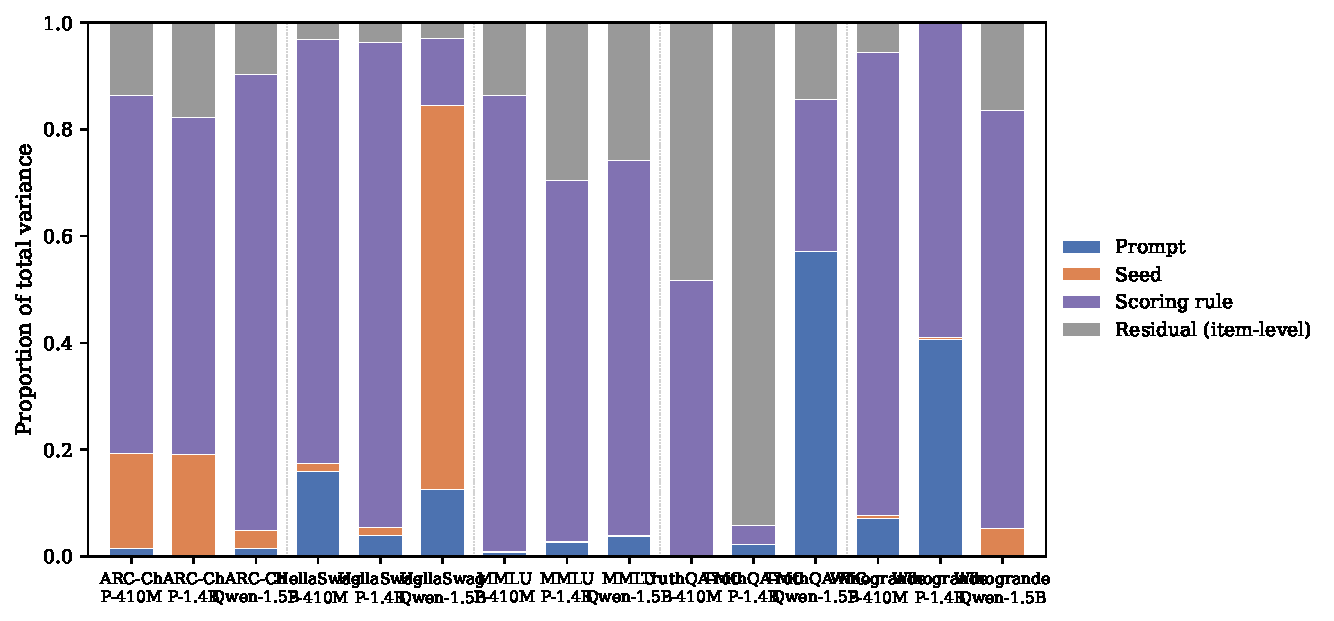
\includegraphics[width=0.98\textwidth]{variance_components_stacked.pdf}
\caption{Per-cell variance components: aggregated decomposition of item-level binary correctness variance into prompt, seed, scoring rule, and residual (item-level) sources, for the fifteen $5 \times 3$ (benchmark, model) cells of the primary panel. Cells are grouped by benchmark; within each benchmark, cells are ordered by model (Pythia-410M, Pythia-1.4B, Qwen2.5-1.5B-Instruct). Scoring-rule variance dominates in twelve of fifteen cells with proportions ranging from $0.28$ (TruthfulQA-MC, Qwen) to $0.91$ (HellaSwag, Pythia-1.4B); the three exceptions are HellaSwag/Qwen (seed dominates at $72\%$), TruthfulQA-MC/Pythia-1.4B (item-level residual dominates at $94\%$), and TruthfulQA-MC/Qwen (prompt dominates at $57\%$). Variance proportions sum to $1.0$ per cell to within machine precision.}
\label{fig:variance-stacked}
\end{figure}

\subsection{Generalizability coefficients}
\label{sec:generalizability-results}

The generalizability coefficient $g$ \citep{brennan2001gtheory, shrout1979icc} estimates the proportion of total observable variance attributable to systematic between-cell differences --- the inferential target the framework's reliability defense (§\ref{sec:reliability-machinery}) holds the score accountable to. Table~\ref{tab:generalizability} reports per-benchmark $g$ under four averaging schemes derived from the variance-components decomposition of §\ref{sec:variance-components-results}: single-occasion ($g_{\mathrm{single}}$, $k = 1$), within-rule averaging across prompts and seeds ($g_{\mathrm{within\text{-}rule}}$), prompt-averaging across the rule and seed facets ($g_{\mathrm{prompt\text{-}avg}}$), and full-design averaging over all admissible conditions per cell ($g_{\mathrm{full}}$).

The pre-registered H2 decision rule (§\ref{sec:design-decisions}) required at least three of five primary benchmarks to have a single-occasion generalizability coefficient below $0.80$. The observed values are: ARC-Challenge $0.564$, HellaSwag $0.953$, MMLU panel $0.301$, TruthfulQA-MC $0.049$, and Winogrande $0.405$. Four of five fall below the threshold; HellaSwag is the exception. H2 is confirmed at $4/5$ where $3/5$ was required.

Averaging across measurement-design facets recovers reliability heterogeneously across benchmarks. ARC-Challenge moves from $g_{\mathrm{single}} = 0.564$ to $g_{\mathrm{full}} = 0.969$, with most of the gain captured by within-rule averaging ($0.877$) --- consistent with the §\ref{sec:variance-components-results} finding that ARC-Challenge's variance is concentrated on the scoring-rule facet, which within-rule averaging absorbs. MMLU panel improves from $0.301$ to $0.981$, with most of the gain coming from prompt-averaging ($0.896$). Winogrande follows a similar pattern at smaller magnitude ($0.405 \to 0.942$). HellaSwag begins above the threshold ($0.953$) and stays there. TruthfulQA-MC is the panel's outlier: it begins below the threshold ($0.049$) and remains below at $g_{\mathrm{full}} = 0.290$. Even averaging over the eight admissible conditions per cell (the seed facet collapses on TruthfulQA-MC, reducing its admissible-condition count to eight), cell-level reliability remains below the conventional $0.80$ standard --- consistent with the §\ref{sec:variance-components-results} attribution of TruthfulQA-MC's variance to item-level residual on the Pythia-1.4B cell ($94\%$) rather than to facets that admissible-design averaging would absorb.

Within the framework's terms, the four-of-five H2 confirmation is the systematic counterpart to the §\ref{sec:tolerance-schedule-results} tolerance result. Where §\ref{sec:tolerance-schedule-results} reports per-cell SEMs that exceed the threshold for second-decimal-precision claims, §\ref{sec:generalizability-results} reports per-benchmark generalizability coefficients that fall below the conventional acceptable-reliability standard. The two findings are not independent: the same variance-components decomposition that produces the SEMs underwrites the $g$ estimates, and a benchmark whose SEM-based tolerance fails the decimal-place test is one whose generalizability under single-occasion measurement is small relative to its measurement-design variance. The schedule and the coefficient are, in measurement-theoretic terms, two readings of the same variance estimate: $g_{\mathrm{single}}$ asks ``what fraction of cell-level variance is the inferential target?'' and the SEM asks ``what cell-level variance does the residual carry?''. Each licenses a different reporting practice --- the coefficient licenses cell-level reliability claims; the SEM licenses decimal-place precision claims --- and the framework's defense holds the report accountable to both.

The TruthfulQA-MC pattern --- $g_{\mathrm{full}} = 0.290$ even under full-design averaging --- is informative for the boundary of the framework's reliability defense. The bounded-precision schedule has an answer for cells where measurement-design averaging recovers reliability (interval-required at single-occasion, possibly two-decimal at full-design); it has a different answer for cells where the residual is so dominant that no admissible-design averaging recovers reliability. On TruthfulQA-MC, cell-level reliability does not get above the threshold under any averaging the panel's measurement universe admits. The schedule treats this as a measurement-instrument finding rather than a model-capability finding: TruthfulQA-MC's $8$-condition cells (seed facet collapsed) cannot, on this regime, support cell-level reliability claims at the conventional standard, regardless of the model under test. A construct-validity reading of the implication (cf.~\citet{bean2025measuring}, §\ref{sec:codev-register}) belongs in §\ref{sec:methodological-implications}; the §\ref{sec:generalizability-results} measurement claim is bounded.

\begin{table}[h]
\centering
\caption{Per-benchmark generalizability coefficients across four averaging schemes derived from the variance-components decomposition. Single-occasion ($k = 1$) measurement falls below the conventional $0.80$ reliability standard for four of five primary benchmarks (H2 confirmed at $4/5$); HellaSwag is the exception. TruthfulQA-MC remains below the threshold under all averaging schemes admissible for its measurement universe (the seed facet collapses on TruthfulQA-MC, reducing its admissible-condition count to eight). $n$~=~3 models per benchmark.}
\label{tab:generalizability}
\begin{tabular}{lcccc}
\toprule
Benchmark & $g_{\mathrm{single}}$ & $g_{\mathrm{within\text{-}rule}}$ & $g_{\mathrm{prompt\text{-}avg}}$ & $g_{\mathrm{full}}$ \\
\midrule
ARC-Challenge & 0.564 & 0.877 & 0.838 & 0.969 \\
HellaSwag     & 0.953 & 0.986 & 0.988 & 0.998 \\
MMLU panel    & 0.301 & 0.600 & 0.896 & 0.981 \\
TruthfulQA-MC & 0.049 & 0.067 & 0.170 & 0.290 \\
Winogrande    & 0.405 & 0.673 & 0.731 & 0.942 \\
\bottomrule
\end{tabular}
\end{table}

\subsection{Tolerance schedule}
\label{sec:tolerance-schedule-results}

The tolerance schedule licenses a per-cell decimal-place reporting precision under the cell's regime classification per the construction in §\ref{sec:tolerance-schedule}. Table~\ref{tab:tolerance-by-cell} reports the schedule across the thirty (model, benchmark, scoring rule) cells of the primary panel; Figure~\ref{fig:tolerance-calibration} plots the schedule's licensed precision against the conventional two-decimal reporting precision typical of recent LLM-evaluation papers.

The cross-model median single-occasion tolerance per benchmark is: ARC-Challenge $0.217$, HellaSwag $0.078$, MMLU panel $0.212$, TruthfulQA-MC $0.596$, and Winogrande $0.126$. The pre-registered H1 decision rule (§\ref{sec:design-decisions}) required at least three of five primary benchmarks to exceed a single-occasion median tolerance of $\pm 0.005$. All five benchmarks exceed the threshold; the bootstrap lower bound on each per-benchmark median also exceeds the threshold. H1 is confirmed at $5/5$ where $3/5$ was required, with the smallest margin (HellaSwag) approximately fifteen-fold above the threshold and the largest (TruthfulQA-MC) approximately one hundred-and-twenty-fold.

At the cell level, single-occasion tolerances range from $0.019$ (HellaSwag, Pythia-1.4B, generate-and-parse, parse-failure-dominated regime) to $0.972$ (TruthfulQA-MC, Pythia-410M, length-normalized log-likelihood, $g$-theory regime). Under the schedule's decimal-place rule, no cell in the primary panel licenses second-decimal reporting at the single-occasion level: every cell's licensed precision is interval-required. Averaging across the full design (twenty-four conditions per cell, eight for TruthfulQA-MC where the seed facet collapses) reduces the per-cell SEM by roughly the square root of the within-cell condition count, and the licensed precision improves accordingly: the per-benchmark medians of full-design tolerance fall to ARC-Challenge $0.044$, HellaSwag $0.016$, MMLU panel $0.019$, TruthfulQA-MC $0.211$, and Winogrande $0.026$. One cell licenses two-decimal reporting under the full-design schedule (HellaSwag, Pythia-1.4B, generate-and-parse, where the parse-failure-dominated regime's cell-SD-based tolerance is small in absolute terms because the cell's score variance is itself small); the remaining twenty-nine cells still require interval reporting at the full-design averaging level.

The thirty cells partition into twenty-three $g$-theory cells and seven parse-failure-dominated cells under the §\ref{sec:design-regime-split} threshold of $0.30$ on median parseability. The parse-failure-dominated cells are concentrated in the generate-and-parse scoring rule on base models (Pythia-1.4B and Pythia-410M); the $g$-theory regime carries the schedule's variance-components-based SEM, while the parse-failure-dominated regime's tolerance is the sample standard deviation of cell scores. The two regimes are reported alongside each other in Table~\ref{tab:tolerance-by-cell} rather than collapsed into a single number; cell-level interpretation routes through the regime classification per §\ref{sec:tolerance-schedule}.

Within the framework's terms, the schedule licenses a specific reading discipline. A reported benchmark score of the form ``$0.74$'' implicitly claims that the second decimal is informative --- that the third digit lies below the standard error of measurement. Under the present panel's measurement universe, that claim is licensed for none of the thirty cells at the single-occasion level and for one of the thirty cells at the full-design level.

The two regimes' tolerance estimates are not interchangeable inferential objects. The $g$-theory regime's tolerance is the variance-components SEM under the declared measurement universe --- how much a cell's score moves under admissible design variation, with the variance attributed to identifiable facets via the mixed-effects cascade of §\ref{sec:design-cascade}. The parse-failure-dominated regime's tolerance is the sample standard deviation of cell scores --- how much a cell's score moves under the variation realized when parse-failure dominates the response distribution. The first is a structural claim about the universe; the second is a dispersion claim about the realized cells. Reporting both rather than collapsing across them is what keeps the cell-level interpretation tractable: a reader interpreting an interval-required cell from the parse-failure-dominated regime is consulting evidence of a different kind than one interpreting an interval-required cell from the $g$-theory regime, and the regime annotation in Table~\ref{tab:tolerance-by-cell} records the difference.

The full-design schedule illustrates the bounded-precision discipline as a measurement-design budget. Recovering second-decimal precision on this regime requires averaging over the full design --- twenty-four condition realizations per cell on the primary panel, eight on TruthfulQA-MC where the seed facet collapses. At that averaging level, one cell licenses two-decimal precision; the remaining twenty-nine still require interval reporting. The schedule does not prohibit second-decimal claims; it specifies the measurement-design cost those claims would require, per cell, under the universe declared. Single-occasion second-decimal claims on this regime are not licensable at any cost, since the SEM at single occasion exceeds $10^{-2}$ for every cell in the panel.

Interval-required reporting is therefore the schedule's default per-cell prescription on this regime, and the form the panel's own results take in Table~\ref{tab:tolerance-by-cell}: every tolerance is reported with its bootstrap lower and upper bound, every cell's licensed precision is named explicitly, and the regime classification is visible per cell rather than averaged away. Whether the same conclusion holds on frontier-scale models, on different benchmark panels, or on adversarial-perturbation universes (cf.~\citet{romanou2026brittlebench}) is a question the schedule defers to re-application under those regimes' own measurement universes; the present finding is bounded to the small-to-mid-scale open-model regime the protocol tests (§\ref{sec:limitations}).

\begin{table}[h]
\centering
\small
\caption{Per-cell tolerance schedule across the thirty (model, benchmark, scoring rule) cells of the primary panel. Single-occasion tolerance corresponds to $k = 1$ measurement; full-design tolerance to averaging over the cell's admissible conditions ($n = 24$ on the four benchmarks where the seed facet contributes, $n = 8$ on TruthfulQA-MC where it collapses). Regime classification (\textit{g} = $g$-theory; \textit{pf} = parse-failure-dominated) follows the §\ref{sec:design-regime-split} threshold of $0.30$ on median parseability. Single-occasion licensed precision is interval-required for all thirty cells. Full-design licensed precision is interval-required for twenty-nine cells; the cell marked $\dagger$ licenses two-decimal-accuracy reporting under full-design averaging. G\&P denotes generate-and-parse; LL denotes length-normalized log-likelihood.}
\label{tab:tolerance-by-cell}
\begin{tabular}{lllcrr}
\toprule
Benchmark & Model & Rule & Regime & Tol.\ (single) & Tol.\ (full) \\
\midrule
ARC-Challenge & Pythia-1.4B  & G\&P & \textit{g}  & 0.188 & 0.038 \\
ARC-Challenge & Pythia-1.4B  & LL   & \textit{g}  & 0.188 & 0.038 \\
ARC-Challenge & Pythia-410M  & G\&P & \textit{g}  & 0.217 & 0.044 \\
ARC-Challenge & Pythia-410M  & LL   & \textit{g}  & 0.217 & 0.044 \\
ARC-Challenge & Qwen2.5-1.5B & G\&P & \textit{g}  & 0.620 & 0.127 \\
ARC-Challenge & Qwen2.5-1.5B & LL   & \textit{g}  & 0.620 & 0.127 \\
HellaSwag     & Pythia-1.4B  & G\&P & \textit{pf} & 0.019 & 0.004$^{\dagger}$ \\
HellaSwag     & Pythia-1.4B  & LL   & \textit{g}  & 0.094 & 0.019 \\
HellaSwag     & Pythia-410M  & G\&P & \textit{pf} & 0.039 & 0.008 \\
HellaSwag     & Pythia-410M  & LL   & \textit{g}  & 0.143 & 0.029 \\
HellaSwag     & Qwen2.5-1.5B & G\&P & \textit{g}  & 0.078 & 0.016 \\
HellaSwag     & Qwen2.5-1.5B & LL   & \textit{g}  & 0.078 & 0.016 \\
MMLU panel    & Pythia-1.4B  & G\&P & \textit{g}  & 0.212 & 0.019 \\
MMLU panel    & Pythia-1.4B  & LL   & \textit{g}  & 0.212 & 0.019 \\
MMLU panel    & Pythia-410M  & G\&P & \textit{pf} & 0.075 & 0.007 \\
MMLU panel    & Pythia-410M  & LL   & \textit{g}  & 0.203 & 0.018 \\
MMLU panel    & Qwen2.5-1.5B & G\&P & \textit{g}  & 0.625 & 0.057 \\
MMLU panel    & Qwen2.5-1.5B & LL   & \textit{g}  & 0.625 & 0.057 \\
TruthfulQA-MC & Pythia-1.4B  & G\&P & \textit{pf} & 0.617 & 0.218 \\
TruthfulQA-MC & Pythia-1.4B  & LL   & \textit{g}  & 0.923 & 0.326 \\
TruthfulQA-MC & Pythia-410M  & G\&P & \textit{pf} & 0.575 & 0.203 \\
TruthfulQA-MC & Pythia-410M  & LL   & \textit{g}  & 0.971 & 0.343 \\
TruthfulQA-MC & Qwen2.5-1.5B & G\&P & \textit{g}  & 0.236 & 0.083 \\
TruthfulQA-MC & Qwen2.5-1.5B & LL   & \textit{g}  & 0.236 & 0.083 \\
Winogrande    & Pythia-1.4B  & G\&P & \textit{pf} & 0.032 & 0.007 \\
Winogrande    & Pythia-1.4B  & LL   & \textit{g}  & 0.453 & 0.093 \\
Winogrande    & Pythia-410M  & G\&P & \textit{pf} & 0.092 & 0.019 \\
Winogrande    & Pythia-410M  & LL   & \textit{g}  & 0.273 & 0.056 \\
Winogrande    & Qwen2.5-1.5B & G\&P & \textit{g}  & 0.126 & 0.026 \\
Winogrande    & Qwen2.5-1.5B & LL   & \textit{g}  & 0.126 & 0.026 \\
\bottomrule
\end{tabular}
\end{table}

\begin{figure}[t]
\centering
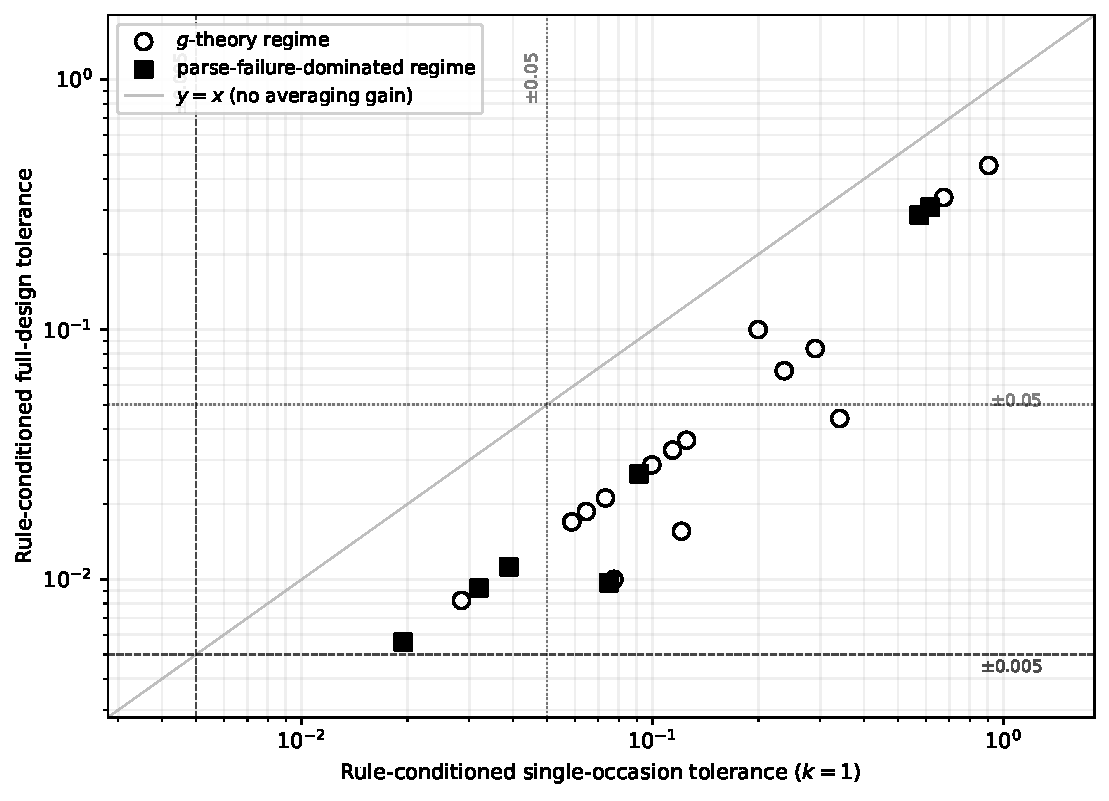
\includegraphics[width=0.78\textwidth]{tolerance_calibration.pdf}
\caption{Tolerance calibration across the thirty cells of the primary panel. X-axis: single-occasion tolerance ($k = 1$); Y-axis: full-design tolerance (averaging over admissible conditions per cell). Both axes log-scaled. Dashed reference lines mark the $\pm 0.005$ threshold (the H1 second-decimal-accuracy boundary); dotted reference lines mark the $\pm 0.05$ threshold (one-decimal accuracy). Cells are colored by regime. No cell falls left of the vertical $\pm 0.005$ line --- zero of thirty cells license second-decimal precision under single-occasion measurement. One cell falls below the horizontal $\pm 0.005$ line: HellaSwag, Pythia-1.4B, generate-and-parse, in the parse-failure-dominated regime, where the cell's small score variance carries small full-design tolerance in absolute terms. The diagonal $y = x$ reference line marks where averaging recovers no precision over single-occasion measurement; every cell sits below the diagonal, with the gap proportional to the full-design averaging gain on the cell.}
\label{fig:tolerance-calibration}
\end{figure}

\subsection{Ranking stability (H3)}
\label{sec:ranking-stability-results}

The pre-registered H3 decision rule (§\ref{sec:design-decisions}) required at least three of five primary benchmarks to have at least one model pair whose pairwise condition-reversal fraction exceeds $20\%$, the threshold raised from an earlier $10\%$ at v1.1-draft to strengthen the test against trivial confirmation. Table~\ref{tab:ranking-reversals} reports per-pair reversal fractions across the three model pairs (Pythia-1.4B vs.\ Pythia-410M, Pythia-1.4B vs.\ Qwen2.5-1.5B-Instruct, and Pythia-410M vs.\ Qwen2.5-1.5B-Instruct) on each of the five primary benchmarks. Each of the five benchmarks has at least one model pair whose condition-reversal fraction exceeds the $20\%$ threshold; H3 is confirmed at $5/5$ where $3/5$ was required.

The reversal pattern across pairs is structurally informative. The within-family Pythia-1.4B vs.\ Pythia-410M pair reverses substantially on every benchmark: $25.0\%$ on ARC-Challenge, $20.8\%$ on HellaSwag, $33.3\%$ on MMLU panel, $50.0\%$ on TruthfulQA-MC ($n = 8$ admissible conditions), and $54.2\%$ on Winogrande. The cross-lineage Pythia-vs-Qwen pairs reverse rarely on the four benchmarks with $n \geq 24$ admissible conditions where the cross-lineage accuracy gap is large: $0\%$ on ARC-Challenge, HellaSwag, and Winogrande for both Pythia models against Qwen; $8.3\%$ and $2.5\%$ on MMLU panel for the Pythia-1.4B vs.\ Qwen and Pythia-410M vs.\ Qwen pairs respectively. TruthfulQA-MC is the exception: its cross-lineage pairs reverse at $37.5\%$ (both pairs), reflecting the small admissible-condition count ($n = 8$) and the small overall mean differences between the cross-lineage pairs ($-0.090$ for Pythia-1.4B vs.\ Qwen, $+0.087$ for Pythia-410M vs.\ Qwen).

The reversal-fraction-vs.-mean-difference relationship is direct on the data. Pairs with overall mean differences below $|0.020|$ (the within-family Pythia pair on ARC-Challenge, HellaSwag, and Winogrande) exhibit reversal fractions of $20\%$ or higher; pairs with mean differences above $|0.20|$ on benchmarks with $n \geq 24$ admissible conditions exhibit reversal fractions below $10\%$. The relationship is what would be expected if condition-level score distributions are roughly the same width across model pairs --- pairs whose mean-difference is small relative to the per-condition score-distribution width have substantial distribution overlap and reverse often, while pairs whose mean-difference exceeds the distribution width reverse rarely.

Within the framework's terms, the H3 result extends the §\ref{sec:tolerance-schedule-results} tolerance finding from per-cell decimal-place licensing to per-pair ranking licensing. A reported leaderboard ranking implicitly claims that the rank order is stable under admissible measurement-design variation. The H3 result reports that this claim fails on close-skill pairs (those whose accuracy gap is small relative to the condition-level score-distribution width) on every benchmark in the primary panel; the rank order between substantively different models (cross-lineage Pythia-vs-Qwen pairs on benchmarks with $n \geq 24$) is stable, and the rank order between similar-capability models (within-family pairs) is not. Aggregate leaderboard reporting that does not separate close-skill comparisons from cross-skill comparisons --- and the field has no current convention for doing so --- does not license rank claims for the close-skill subset on this regime.

\citet{romanou2026brittlebench} report a $63\%$ ranking-reversal rate under any-single-perturbation on frontier-scale models across $26$ benchmarks. The Brittlebench reversal universe is broader than the present paper's (semantics-preserving perturbations on a wider set than community-provenance prompts), and the model regime is different (frontier vs.\ small-to-mid-scale open). The two findings nonetheless align in order of magnitude: under measurement-design variation, leaderboard rankings on a non-trivial fraction of pairs do not reproduce. The present paper's $20\%$-threshold confirmation under a narrower perturbation universe and a different model regime is a regime-bounded instance of the same phenomenon Brittlebench's $63\%$ finding registers at frontier scale.

\begin{table}[h]
\centering
\small
\caption{Per-pair condition-reversal fractions across the three model pairs on the five primary benchmarks. Mean differences ($\bar{\Delta} = \mathrm{accuracy}_A - \mathrm{accuracy}_B$) are aggregated across admissible conditions per (benchmark, pair). The within-family Pythia-1.4B vs.\ Pythia-410M pair reverses substantially on every benchmark; cross-lineage Pythia-vs-Qwen pairs reverse rarely on the four benchmarks with $n \geq 24$ admissible conditions where the cross-lineage accuracy gap is large; TruthfulQA-MC is the exception ($n = 8$, small mean differences). Each benchmark has at least one model pair whose reversal fraction exceeds the pre-registered $20\%$ threshold (H3 confirmed at $5/5$, marked $\checkmark$).}
\label{tab:ranking-reversals}
\begin{tabular}{llrrrc}
\toprule
Benchmark & Pair & $\bar{\Delta}$ & $n$ & Reversal & H3 \\
\midrule
ARC-Challenge & Pythia-1.4B / Pythia-410M  & $+0.010$ & 24  & 0.250 & $\checkmark$ \\
ARC-Challenge & Pythia-1.4B / Qwen2.5-1.5B & $-0.383$ & 24  & 0.000 & \\
ARC-Challenge & Pythia-410M / Qwen2.5-1.5B & $-0.393$ & 24  & 0.000 & \\
HellaSwag     & Pythia-1.4B / Pythia-410M  & $-0.015$ & 24  & 0.208 & $\checkmark$ \\
HellaSwag     & Pythia-1.4B / Qwen2.5-1.5B & $-0.430$ & 24  & 0.000 & \\
HellaSwag     & Pythia-410M / Qwen2.5-1.5B & $-0.415$ & 24  & 0.000 & \\
MMLU panel    & Pythia-1.4B / Pythia-410M  & $+0.034$ & 120 & 0.333 & $\checkmark$ \\
MMLU panel    & Pythia-1.4B / Qwen2.5-1.5B & $-0.208$ & 120 & 0.083 & \\
MMLU panel    & Pythia-410M / Qwen2.5-1.5B & $-0.242$ & 120 & 0.025 & \\
TruthfulQA-MC & Pythia-1.4B / Pythia-410M  & $-0.177$ & 8   & 0.500 & $\checkmark$ \\
TruthfulQA-MC & Pythia-1.4B / Qwen2.5-1.5B & $-0.090$ & 8   & 0.375 & $\checkmark$ \\
TruthfulQA-MC & Pythia-410M / Qwen2.5-1.5B & $+0.087$ & 8   & 0.375 & $\checkmark$ \\
Winogrande    & Pythia-1.4B / Pythia-410M  & $-0.012$ & 24  & 0.542 & $\checkmark$ \\
Winogrande    & Pythia-1.4B / Qwen2.5-1.5B & $-0.230$ & 24  & 0.000 & \\
Winogrande    & Pythia-410M / Qwen2.5-1.5B & $-0.218$ & 24  & 0.000 & \\
\bottomrule
\end{tabular}
\end{table}

\subsection{MMLU subject-decomposition case (H4)}
\label{sec:mmlu-subjects-results}

The pre-registered H4 decision rule (§\ref{sec:design-decisions}) required the model-by-subject interaction in the MMLU subject panel to explain at least $10\%$ of total item-level response variance after controlling for model main effect and subject main effect, indicating that collapsed ``MMLU accuracy'' would mask meaningful model-specific subject variation. The observed interaction proportion is $0.0046$ --- approximately a twentieth of the pre-registered threshold value. H4 is not confirmed.

The pre-registered null reads as a substantive measurement finding. Subject-level differences in MMLU performance on this panel are dominated by additive main effects: subject difficulty (some subjects are uniformly harder) and model capability (some models are uniformly stronger), with model-specific subject interactions contributing approximately one-half of one percent of total variance. The five-subject panel was pre-registered at lock time to mitigate small-model floor risk (one subject from each MMLU subject grouping, chosen to span difficulty rather than to maximize between-model differentiation); the null result indicates that the additive main-effects structure captures most of the observable variance on this panel-and-regime configuration, not that the null would necessarily replicate on a different subject panel or model regime.

Within the framework's terms, the H4 null is informative for the §\ref{sec:reliability-machinery} reliability defense in a specific way: the subject facet does not introduce additional model-specific variance on this regime that the §\ref{sec:variance-components-results} cascade did not already estimate at the panel level. Collapsed ``MMLU accuracy'' on this regime --- aggregated across the five locked subjects --- is not, on the present panel, masking heavy subject-by-model heterogeneity. The framework's per-cell reliability picture (§\ref{sec:tolerance-schedule-results}) does not need to be further disaggregated to a per-subject level on this regime; the panel-level cells remain the appropriate unit of measurement-tolerance reporting on the small-to-mid-scale open-model regime tested.

The pre-registered subject choice constrains the scope of the null. The five subjects (\texttt{world\_religions}, \texttt{elementary\_mathematics}, \texttt{high\_school\_psychology}, \texttt{professional\_accounting}, \texttt{global\_facts}) were chosen for floor-risk mitigation on small models, not to maximize between-model differentiation. A subject panel chosen to maximize differentiation, or a model regime where capability differences interact with subject domain (e.g., frontier-scale models with substantial domain specialization), would test a different question. Whether the null transfers to those regimes is named in §\ref{sec:future-work}; the present null is bounded to the panel and regime declared. The pre-registered framework treats a confirmed hypothesis and a pre-registered null as equal-weight reportable findings, neither over-interpreted as confirmation nor apologized for as a missed effect.

% TABLE 6 PLACEHOLDER. Per-subject variance components within MMLU panel,
% with regime classification. 5 subjects × 4 facets = 20 rows.

% FIGURE 5 PLACEHOLDER. Subject-level forest plot: point estimate ± SEM per
% (model, subject), showing where within-MMLU subject variance dominates between-
% subject signal vs. where additive main effects capture most of the variance.

\subsection{GSM8K case}
\label{sec:gsm8k-results}

GSM8K is reported as a single-model case study on Pythia-1.4B following the v1.1.2 budget amendment (\texttt{LOCK\_NOTES.md}; see also §\ref{sec:design-regime-split}). Pythia-410M's and Qwen2.5-1.5B-Instruct's $48$ GSM8K conditions were dropped via the pre-committed cost-projection tripwire; the case-study scope is preserved at $24$ admissible conditions on Pythia-1.4B (four prompt templates $\times$ three seeds $\times$ two extraction variants). What is given up is the cross-model comparison originally planned for the secondary tier; what remains is the within-model regime-split demonstration the §\ref{sec:design-materials} measurement universe articulates GSM8K as a vehicle for.

The two extraction variants test the framework's regime split (§\ref{sec:design-regime-split}) directly. The strict extraction (exact-match against the post-``\#\#\#\#'' digit sequence) yields a per-cell SEM of $0.0015$ and a tolerance of $0.0030$, below the $0.005$ H1 threshold; the schedule licenses two-decimal-accuracy reporting under strict extraction. The permissive extraction (a regex accepting common formatting variants) yields a per-cell SEM of $0.0036$ and a tolerance of $0.0071$, above the threshold; the schedule's licensed precision under permissive extraction is interval-required.

Within the framework's terms, the strict-vs-permissive contrast is the regime split at its most visible operationalization: the same benchmark, on the same model, on the same item set, with the same prompts, produces different licensed reporting precisions under different extraction rules. The extraction rule is not, on GSM8K, a transparent post-hoc choice of how to summarize a stable score; it is part of the measurement instrument, and the variance estimates that drive the schedule depend on which instrument is being used. A GSM8K accuracy report that does not declare its extraction rule is, in the framework's terms, a measurement without a fully-stated measurement universe.

This is a finding the framework's reproducibility-and-pre-registration discipline surfaces in the same epistemic register as the pre-registered regime split itself --- discovery-like in the narrower reporting sense that the precursor paper articulates \citep{anonymized2026n134}. A study committing to a single extraction rule without observing the parseability distribution would not have surfaced the regime split's effect on tolerance on this benchmark; a study reporting only a single point estimate without naming the extraction rule would not have surfaced the dependence on it. The cross-model comparison originally planned would have made the within-model demonstration visible alongside the across-model contrast; the budget-driven scope reduction preserves the within-model demonstration the case study is empirically anchored to, and the cross-model extension is named in §\ref{sec:future-work}.

% TABLE 7 PLACEHOLDER. GSM8K outcomes for Pythia-1.4B across (prompt, seed,
% extraction variant) cells: parseability rate, accuracy, regime classification.
% Source: analysis/gsm8k_case/gsm8k_tolerance_schedule.csv.

% FIGURE 6 PLACEHOLDER. Parseability rate distribution per (prompt × seed) on
% Pythia-1.4B; argues empirically for the 0.30 threshold or against it on the
% single-model evidence base.

\section{Discussion}
\label{sec:discussion}

% EDIT: 2026-04-28 — §8 drafted post-Phase-5. Five subsections: methodological
% EDIT: implications (the field-level reading-discipline move), limitations
% EDIT: (within-paper), relationship to precursor paper (cross-paper substrate-
% EDIT: portability move; load-bearing for §1.3 contribution claim 1), future
% EDIT: work, anticipated objections. Cross-paper register convergences with
% EDIT: N134 are intentional per CLAUDE.md program conventions.

\subsection{Methodological implications}
\label{sec:methodological-implications}

The empirical findings reported in §\ref{sec:results} license a specific reading discipline for benchmark accuracy reports under measurement universes structurally similar to the present panel's. The discipline is local to the framework's bounded-precision claim: it does not retroactively re-adjudicate published numbers or claim that any specific report is defective; it specifies what credence a careful reader is now licensed to place in benchmark numbers reported under conditions the present study's measurement universe matches.

The reading-discipline implication is direct. A benchmark-accuracy report at two-decimal precision under single-occasion measurement on the small-to-mid-scale open-model regime, evaluated on benchmarks within the primary panel, claims a precision the schedule does not license: thirty of thirty cells in the panel require interval reporting at single-occasion. The implication generalizes to the field as a function of how closely a given report's measurement universe matches the panel's: a report that names its prompt template, seed, scoring rule, and measurement universe explicitly, under conditions structurally similar to the panel, inherits the panel's licensed-precision finding. A report that does not name those elements is, in the framework's terms, a measurement without a stated measurement universe; the schedule cannot speak to its licensed precision because the universe is undeclared.

The H2 four-of-five generalizability finding sharpens the implication. Single-occasion generalizability below the conventional $0.80$ standard means that the cell-level reliability of single-occasion measurement is small relative to its measurement-design variance: a model-pair comparison, a leaderboard ranking, or any inference that treats a single-occasion score as a reliable estimate of the cell-level reliable score is, on this regime, drawing inference from a measurement instrument the framework's reliability defense flags as inadequate to the precision claimed. Recovering reliability requires averaging over admissible measurement-design variation per cell; the §\ref{sec:tolerance-schedule-results} schedule reports what averaging level recovers what precision and the design budget that imposes per cell.

A vocabulary note connects the schedule's reliability machinery to the broader measurement-discipline register the §\ref{sec:codev-register} corpus has developed. \citet{heineman2025signal}'s \emph{signal} quantity --- the ratio of systematic between-model variance to total variance --- maps onto what the generalizability-theory tradition calls the \emph{generalizability coefficient}; the two are the same object expressed in different methodological registers. The tolerance-schedule prescription sits cleanly on top of either register: the schedule converts the variance-components SEM (or, equivalently, the cell-level $1 - g_{\mathrm{single}}$ relative to total variance) into licensed decimal-place precision via the §\ref{sec:tolerance-schedule} decimal-place rule. A reader more comfortable with the signal-and-noise vocabulary of \citet{heineman2025signal} can read the present paper's $g$ coefficients as the corresponding signal estimates without loss; the methodological-register choice does not change the substantive measurement claim.

The H3 ranking-stability finding pulls the implication into a register the field's reporting practice does not currently distinguish. Ranking instability is concentrated on close-skill model pairs --- pairs whose accuracy gap is small relative to the per-condition score-distribution width --- and rank stability holds on cross-skill pairs. A leaderboard comparison between substantively different models (the cross-lineage Pythia-vs-Qwen pairs in the present panel on benchmarks with $n \geq 24$ admissible conditions) is licensed at single-occasion measurement; a leaderboard comparison between similar-capability models (the within-family Pythia pair) is not. Field-level leaderboards do not currently visibly separate close-skill from cross-skill comparisons; the H3 finding licenses the prescriptive recommendation that a leaderboard-aware reading discipline ask, of any reported model-pair comparison, what the per-condition score-distribution overlap between the pair is. Where the overlap is substantial, the rank claim is not licensed at single-occasion measurement under this regime.

The H4 null adds a register-bounded note: subject-level decomposition of the MMLU panel's variance does not show heavy model-by-subject heterogeneity on this regime, which means the per-cell reliability picture (§\ref{sec:variance-components-results}) is the appropriate level at which to evaluate MMLU measurement reliability on this panel. A panel chosen for differentiation rather than floor-risk mitigation, or a frontier-scale model regime where subject specialization may interact with model capability, would test a different question; whether the additive-main-effects structure transfers to those regimes is named in §\ref{sec:future-work}.

\subsection{Limitations}
\label{sec:limitations}

The study's empirical claims are bounded to the regime its protocol tests. The primary panel is small-to-mid-scale open language models (Pythia-410M, Pythia-1.4B, Qwen2.5-1.5B-Instruct); the framework's findings on tolerance, generalizability, and ranking stability are not extrapolated to frontier-scale models. The empirical pattern --- scoring-rule dominance of variance, regime split between $g$-theory and parse-failure-dominated cells, close-skill ranking instability --- may transfer to frontier-scale evaluation, may not, or may transfer with quantitatively different magnitudes. The framework is what is offered for re-application; the specific schedules and coefficients are regime-bounded.

The benchmark panel is six benchmarks (five primary plus GSM8K as a single-model case), not the full LLM benchmark landscape. The five primary benchmarks span constrained-choice reasoning across knowledge domains, commonsense, factuality, and scientific reasoning, and the panel is large enough to test the H1--H4 decision rules at the pre-registered thresholds; it is not large enough to license generalization to benchmark domains the panel does not include. Long-context reasoning, code generation, mathematical theorem-proving, and adversarial-perturbation universes are out of scope; whether the framework's decimal-place schedule transfers cleanly to those domains is named in §\ref{sec:future-work}.

The measurement universe declared in §\ref{sec:design-materials} is constrained by design. Benchmark contamination, agentic-evaluation tasks, chain-of-thought scoring rules, and adversarial-perturbation prompt families are not part of the universe. Each is a separate measurement question that the present framework does not estimate; the framework's prescription is bounded to the universe it does estimate.

The mixed-effects cascade is high-capacity relative to per-cell $N$. The random-effects structure pre-registered at v1.1.2 has approximately a dozen named effects (prompt, seed, scoring rule, item, model-prompt and model-scoring-rule interactions) fit on cells with $24$ admissible conditions (eight on TruthfulQA-MC). The cascade is appropriate for testing whether the framework's variance-decomposition machinery surfaces measurement structure on this substrate; it is not appropriate as a deployable accuracy predictor, and no such predictor is offered. The same epistemic move appears on the precursor paper's substrate at corresponding scale (cf.~\citet{anonymized2026n134}, where the family-pair residualization is acknowledged as a high-capacity baseline by design); both papers' high-capacity caveats are the same kind of limitation, not different ones.

The three-model panel is not a population. Two of the three models are same-family (Pythia-410M and Pythia-1.4B); the third (Qwen2.5-1.5B-Instruct) is a single cross-lineage point. Pattern-level findings about within-family vs.\ cross-lineage ranking stability rest on a single cross-lineage axis; whether the pattern extends across other lineage pairs is empirically open. The variance-components decomposition's facet attributions are estimated per (benchmark, model) cell, and the H2 generalizability coefficients are aggregated at the benchmark level across the three models; readers should not read either as licensing claims about the population of small-to-mid-scale open models in general.

\subsection{Relationship to the precursor paper}
\label{sec:relationship-to-precursor}

Contribution claim 1 (§\ref{sec:contributions}) rests on the empirical demonstration that the four-component measurement-discipline framework survives application to a substrate structurally different from the one it was developed on. The precursor paper \citep{anonymized2026n134} applied the framework to LoRA-merging diagnostic correlations on $n = 45$ cross-task adapter pairs, scored via partial Spearman with cross-seed ICC reliability and family-pair confound decomposition; the present paper applies it to LLM benchmark accuracy on item-level binary correctness across thousands of items per cell, scored via mixed-effects variance-components GLMM with bootstrap CIs on per-cell SEM and pre-registered random-effects structure. The substrates differ on inferential target (regression-coefficient correlation vs.\ classification accuracy), scoring object (continuous Spearman correlations vs.\ binary item correctness), sample-size regime ($n = 45$ pairs vs.\ thousands of items per cell), error structure (cross-seed ICC vs.\ mixed-effects variance components), and adversary class (subspace-vs-cosine alignment vs.\ scoring-rule choice and prompt-format variation). Surviving application to both, with pre-registered findings on each, is non-trivial evidence that the framework is portable across the kinds of structural variation the field's substrates actually exhibit.

The two papers' joint empirical content is what makes the portability claim defensible. The precursor paper's substantive findings include a pre-registered H1 null on its substrate (no LoRA-vs-full-FT advantage in the regime tested), a rank-on-residuals observation surfaced by the framework's discipline (a measurement constraint not visible without the framework's audit-trail commitments), and qualitative reproducibility of the analysis chain on a follow-up substrate. The present paper's findings include H1, H2, and H3 confirmed; H4 not confirmed (a pre-registered null with the same epistemic register as the precursor's H1 null); bit-identical reproducibility of the canonical analysis run; and the parse-failure regime split as a measurement-instrument finding on the present paper's substrate, with the GSM8K extraction-rule sensitivity (§\ref{sec:gsm8k-results}) as a within-benchmark instance. The combined pattern --- pre-registered methodology surfacing both confirmations and pre-registered nulls on both substrates, with substrate-specific findings (rank-on-residuals on one, regime split and extraction-rule sensitivity on the other) the framework's discipline made visible --- is what the substrate-portability claim references empirically.

The framework's component practices are, taken individually, the standard stock of classical test theory and generalizability theory: variance-components decomposition, ICC, generalizability coefficients, bounded-precision logic, pre-registered confound enumeration. The framework's claim is that they are jointly required, not that any individual one is novel. A reader who would dispute the portability claim by pointing at the methodological standardness of any individual component is not reading the contribution claim correctly: the claim is that the joint discipline survives application to a substrate structurally different from the one it was developed on, not that any individual technique is new. Two demonstrations is not $k = \infty$ portability, and neither paper claims it; the claim is that two demonstrations on appropriately diverse substrates is enough evidence to establish that the framework is not silently overfit to the substrate it was developed on.

The cross-paper coordination at the phrasing level of certain registers is part of the program's coherence rather than coincidence. The ``discovery-like in the narrower reporting sense'' framing applied to the rank-on-residuals observation in the precursor paper and to the regime split here, the post-hoc analysis register naming exploratory findings as ``hypothesis-generating rather than confirmatory evidential status,'' and the high-capacity-baseline acknowledgment for the family-pair residualization on one substrate and the mixed-effects cascade on the other --- these are intentionally consistent across the two papers. The joint reading the two papers license is that the framework's discipline produces findings of a specific epistemic kind on both substrates, with consistent register across cases, even though the substrates' empirical content is paper-specific.

\subsection{Future work}
\label{sec:future-work}

Five extensions are named here; each preserves the framework's discipline while expanding the regime tested.

\textbf{Frontier-scale extension.} The present paper's primary panel is small-to-mid-scale open models. Re-applying the framework to frontier-scale models on the same benchmark panel would test whether the H1--H3 confirmations transfer; the H4 null may be regime-specific and would benefit from frontier-scale re-estimation. The methodological-tooling cost is modest (the pipeline is regime-portable); the GPU cost is the limiting factor.

\textbf{Chain-of-thought and reasoning-trace scoring.} The present paper's two scoring rules (length-normalized log-likelihood, generate-and-parse) test constrained-choice operationalizations of the benchmark task. A chain-of-thought scoring rule operationalizes a different aspect of the underlying capability (multi-step reasoning quality vs.\ end-state correctness) and is the subject of substantial active debate in the field. The framework's apparatus extends cleanly: the chain-of-thought rule joins the scoring-rule facet of the variance-components decomposition, with the rule's contribution to total variance estimable per cell. The methodological commitment is the same; the empirical content is open.

\textbf{IRT-style item-level decomposition.} The present paper's mixed-effects cascade treats items as a random effect within benchmarks; an item-response-theory extension (cf.~\citet{sui2025evaluating} on LLM-as-rater MFRM) would estimate per-item difficulty and discrimination parameters and license per-item contribution to the cell-level reliability picture. The IRT extension would substantively refine the per-cell tolerance schedule by separating item-level variance from instrument-level variance more finely than the present cascade does.

\textbf{Adversarial-perturbation universe.} The present paper's measurement universe is community-provenance prompt variation; \citet{romanou2026brittlebench}'s perturbation universe is broader (semantics-preserving perturbations on a wider set of prompt forms). The two universes are complementary: community-provenance variation tests admissible measurement-design variation in the field's actual reporting practice, while adversarial perturbation tests model robustness to what an adversarially-minded measurement designer could try. A paper extending the framework's tolerance schedule across both universes would license a richer per-cell precision-licensing story.

\textbf{Cross-model GSM8K and other open-generation benchmarks.} The §\ref{sec:gsm8k-results} case study is single-model on Pythia-1.4B following the v1.1.2 budget amendment. A cross-model extension on GSM8K, plus extensions to other open-generation benchmarks (BIG-Bench Hard sub-tasks, open-ended summarization with reference-based scoring, code generation with execution-based scoring), would substantially broaden the regime-split evidence base.

The list is constrained to extensions the framework's apparatus directly supports; methodologically orthogonal future work (contamination-aware extension, agentic-evaluation extension, model-internals interpretability extension) is named in the field's broader future-work register but is not internal to the present framework's discipline.

\subsection{Anticipated objections}
\label{sec:anticipated-objections}

Four reviewer objections are predictable on the present paper; each is addressed in two-to-three sentences in the same register the precursor paper used (cf.~\citet{anonymized2026n134}).

\textbf{``Two demonstrations is not a substrate-portability test.''} The defense is recorded in §\ref{sec:contributions} contribution claim 1 and §\ref{sec:relationship-to-precursor}: the precursor paper's substrate (LoRA-merging diagnostic correlations on $n = 45$ cross-task pairs) and the present paper's substrate (item-level binary correctness across thousands of items per cell) differ on inferential target, scoring object, sample-size regime, error structure, and adversary class. Two demonstrations on substrates this structurally different is non-trivial evidence of portability; we do not claim $k = \infty$ portability, and neither does the precursor.

\textbf{``The small-to-mid-scale open-model regime does not extrapolate to frontier.''} The pre-registered scope is exactly the regime tested. The framework is what is offered for re-application; the specific tolerance schedule and generalizability coefficients are regime-bounded. Whether the same conclusions hold at frontier scale is named in §\ref{sec:future-work} as the first listed extension; the present paper does not claim frontier-scale generalization.

\textbf{``The regime split (D-09 $\to$ v1.1.2) was added after data collection began and looks ad-hoc.''} The regime split was added before any analysis was run, in response to two events: the daily-review-surfaced publication of NIST AI 800-3 \citep{nist2026statmodels} formally endorsing GLMM for variance decomposition on AI benchmarks (February 2026), and early Phase~4 GPU output showing that approximately one-fifth of the cells in the primary panel sit outside the parseability range where GLMM and the linear probability model substantially agree. The amendment is recorded in \texttt{LOCK\_NOTES.md} v1.1.2 with full audit, the parseability threshold ($0.30$) is a pre-specified parameter rather than a tuned one, and the split is justified as a response to a methodological tension (NIST endorsing GLMM on cells where LPM and GLMM diverge) rather than as a fit-the-data move. The cross-paper register convention --- ``discovery-like in the narrower reporting sense'' --- is what the regime split is offered in: a measurement constraint surfaced by the framework's discipline that would not be visible in a study committing to a single variance-decomposition method without observing the cell-level parseability distribution.

\textbf{``No contamination assessment.''} Correct. Benchmark contamination is a separate (and well-studied; e.g., \citet{hasan2025pitfalls}) measurement question. The present paper's measurement universe is admissible-prompt-and-scoring-rule variation conditional on a fixed item set; whether the item set itself is contaminated is orthogonal to the variance decomposition the framework estimates. Contamination-aware extension is named in §\ref{sec:future-work} as adjacent future work; the framework's apparatus does not extend cleanly to it (contamination detection requires different methodological tools than measurement-design variance estimation), and the present paper makes no contamination-related claim.

\section{Conclusion}
\label{sec:conclusion}

This paper applies a four-component measurement-discipline framework --- construct articulation, reliability estimation, precision and tolerance, pre-registered confound decomposition --- to LLM benchmark evaluation on a small-to-mid-scale open-model regime. Three of four pre-registered hypotheses were confirmed: single-occasion tolerance exceeds the second-decimal-precision threshold on all five primary benchmarks (H1, $5/5$); single-occasion generalizability falls below the conventional $0.80$ reliability standard on four of five (H2, $4/5$); each primary benchmark has at least one model pair whose ranking does not survive admissible measurement-design variation (H3, $5/5$). The fourth hypothesis was not confirmed: the MMLU subject panel's model-by-subject interaction proportion is approximately a twentieth of the threshold value, indicating that subject-level variation on this panel is dominated by additive main effects (H4, pre-registered null). The paper's distinctive prescriptive contribution within the co-developed measurement-discipline register is the decimal-place precision tolerance schedule (§\ref{sec:tolerance-schedule}), which licenses what numerical precision a reported score actually supports under a declared measurement universe. The present panel's schedule licenses interval-required reporting for thirty of thirty cells at single-occasion measurement and for twenty-nine of thirty at full-design averaging; recovering second-decimal precision under this regime requires averaging across the full measurement design, with the budget that imposes per cell.

The paper is the second worked demonstration of the framework, on a substrate (LLM benchmark evaluation) deliberately chosen to be structurally different from the framework's first demonstration on LoRA-merging diagnostics \citep{anonymized2026n134}. The two demonstrations' joint empirical content --- both pre-registered methodologies producing confirmations and pre-registered nulls, both surfacing substrate-specific measurement-instrument findings the framework's discipline made visible (rank-on-residuals on one substrate, regime split and extraction-rule sensitivity on the other) --- is what the §\ref{sec:contributions} substrate-portability claim references. Two demonstrations is not portability without bound; it is enough to establish that the framework is not silently overfit to the substrate it was developed on.

% =============================================================================
% Appendices
% =============================================================================

\appendix

\section{Pre-registration record (selected sections)}
\label{app:prereg}

This appendix reproduces the load-bearing sections of the locked pre-registration document at lock state v1.1.2 (config hash \texttt{fbc4a5dd}). The full pre-registration document, including procedural sections (timeline, budget, deliverables) and historical-record sections (version history with internal-review decisions), is available in the supplementary materials and at the repository tag \texttt{v1\_1\_2\_LOCKED}. Sections reproduced below: the version history naming the lock-amendment chain (§\ref{app:prereg-version-history}); the pre-registered hypotheses and decision rules (§\ref{app:prereg-hypotheses}); the measurement universe and admissibility rules (§\ref{app:prereg-universe}); materials (§\ref{app:prereg-materials}); design and data hierarchy (§\ref{app:prereg-design}); pre-registered analyses (§\ref{app:prereg-analyses}); and the deviations protocol (§\ref{app:prereg-deviations}). Sections omitted: §1 Purpose (duplicates main-body §\ref{sec:intro}), §2 Theoretical framing (duplicates §\ref{sec:framework}), §8 Confound decomposition (duplicates §\ref{sec:confound-decomposition}), §9 Scope claims (duplicates §\ref{sec:scope} and §\ref{sec:limitations}), §10 Timeline and budget (operational), §12 Deliverables (operational), §14 Open Questions for Internal Review (resolved at v1.1-draft).

\subsection{Version history}
\label{app:prereg-version-history}

\textbf{v1 (2026-04-24):} initial draft protocol. Two-tier design (constrained-choice primary, open-generation secondary). Instruction-tuned model included. MMLU operationalized as a pre-registered subject panel rather than as the full benchmark. Tolerance schedule formulated with explicit decimal-place precision logic.

\textbf{v1.1-draft (2026-04-24):} research decisions resolved following internal review. (i) MMLU subject panel finalized: \texttt{world\_religions}, \texttt{elementary\_mathematics}, \texttt{high\_school\_psychology}, \texttt{professional\_accounting}, \texttt{global\_facts}; STEM and professional slots substituted to reduce small-model floor risk. (ii) Instruction-tuned model locked to Qwen2.5-1.5B-Instruct. (iii) GSM8K extraction variants remain two (strict $+$ permissive); chain-of-thought scoring deferred to future work. (iv) H3 ranking-reversal threshold raised from $10\%$ to $20\%$ to strengthen the decision rule against trivial-confirmation objection.

\textbf{v1.1-LOCKED (2026-04-25):} all operational items resolved: 24 prompt files sourced from canonical community repositories; 3 model HF revisions pinned; 6 dataset version hashes pinned; 24 prompt content hashes computed; admissibility statuses promoted from \texttt{draft} to \texttt{locked}; \texttt{00\_validate\_config.py} reports 0 errors, 0 warnings; config hash \texttt{65fdd1c2}.

\textbf{v1.1.1-LOCKED (2026-04-25):} Phase 3 dry-run amendments. Winogrande \texttt{item\_id\_field} corrected from \texttt{qID} (does not exist on the HF dataset) to \texttt{sentence}; tier filter excluding GSM8K from few-shot draws removed. Both fixes applied before any data was collected. Config hash \texttt{89ce3f1f}.

\textbf{v1.1.2-LOCKED (2026-04-26):} regime-split resolution of D-09 (LPM-not-logistic deviation). NIST AI 800-3 (February 2026) endorsement of GLMM and preliminary GPU-run parseability data motivated the amendment. Added \texttt{tolerance.parse\_failure\_threshold = 0.30}; cells below threshold route to sample-SD-based tolerance. Pre-registered hypothesis tests unchanged; the seven load-bearing pre-registered commitments unchanged. Config hash \texttt{fbc4a5dd}.

\subsection{Pre-registered hypotheses and decision rules}
\label{app:prereg-hypotheses}

\textbf{Primary research question.} Under admissible variation in prompt template, few-shot exemplar selection, and scoring rule, how reliable are benchmark accuracy scores for small-to-mid-scale open language models on a fixed panel of constrained-choice benchmarks, and what decimal-place precision do they support in reporting?

\textbf{H1 (primary; tolerance schedule).} For at least three of the five benchmarks in the primary panel, the median single-occasion tolerance across the three primary models exceeds $\pm 0.005$ accuracy ($\pm 0.5$ percentage points), making second-decimal reporting questionable and third-decimal reporting unsupported under the decimal-place decision rule.

\textbf{H2 (generalizability).} For at least three of the five primary benchmarks, the generalizability coefficient under single-occasion measurement (single prompt $\times$ single seed $\times$ single scoring rule) is less than $0.80$, indicating that single-occasion evaluation is an unreliable estimator of the generalized score.

\textbf{H3 (ranking stability).} For at least two of the five primary benchmarks, the fraction of condition-pair ranking reversals between any two of the three tested models exceeds $20\%$, indicating that single-occasion comparisons between models are not stable. Threshold raised from $10\%$ to $20\%$ at v1.1-draft to strengthen the decision rule against trivial confirmation.

\textbf{H4 (MMLU subject interaction).} The MMLU subject-panel model $\times$ subject interaction explains $\geq 10\%$ of total item-level response variance (after controlling for model main effect and subject main effect), indicating that collapsed ``MMLU accuracy'' masks meaningful model-specific subject variation.

\textbf{Decimal-place decision rule (tolerance schedule).} A reported decimal place at precision $p$ is licensed under these data only if the estimated measurement tolerance ($2 \times$ single-occasion SEM) is less than half a unit at that place. Two decimals (e.g., $0.74$) require tolerance $< \pm 0.005$; three decimals (e.g., $0.742$) require tolerance $< \pm 0.0005$; one decimal in percentage form ($74.2\%$) requires tolerance $< \pm 0.05$ percentage points; integer percent ($74\%$) requires tolerance $< \pm 0.5$ percentage points. The tolerance schedule produced by this study is the empirical instantiation of this rule for each (benchmark, model) cell in the primary panel.

\subsection{Measurement universe and admissibility rules}
\label{app:prereg-universe}

A measurement condition (prompt template, few-shot exemplar draw, scoring rule) is admissible for inclusion in the measurement universe of a benchmark if and only if it satisfies all of the following:

\textbf{1. Task preservation.} The condition's prompt preserves the benchmark's intended task, answer space, and instruction semantics.

\textbf{2. Community provenance.} The condition is traceable to a community source: the benchmark authors' original prompt, a standard evaluation-harness default (e.g., \texttt{lm-evaluation-harness}), a published variant in a peer-reviewed evaluation paper, or the HELM reference prompt. Novel prompts constructed \emph{de novo} for this study are not admissible.

\textbf{3. Scoring-rule fidelity.} The scoring rule correctly identifies the benchmark's intended answer under its operationalization. Log-likelihood scoring over answer choices and generate-and-parse scoring with regex extraction are both admissible for constrained-choice benchmarks; ad-hoc LLM-as-judge scoring is not admissible in the primary study.

For each benchmark in the primary panel, the measurement universe is four admissible prompt templates (P1: original benchmark authors; P2: \texttt{lm-evaluation-harness} default; P3: HELM reference or published variant; P4: minimal direct-instruction variant) $\times$ three few-shot exemplar seeds (42, 123, 2024) $\times$ two scoring rules (length-normalized log-likelihood and generate-and-parse). The nominal admissible-condition count per (benchmark, model) cell is $4 \times 3 \times 2 = 24$, reduced where a facet collapses (TruthfulQA-MC collapses the seed facet to a single level at $0$-shot).

\subsection{Materials}
\label{app:prereg-materials}

\textbf{Models (three primary):} Pythia-410M (\texttt{EleutherAI/pythia-410m} at HF revision \texttt{9879c9b5}), Pythia-1.4B (\texttt{EleutherAI/pythia-1.4b} at \texttt{fedc38a1}), Qwen2.5-1.5B-Instruct (\texttt{Qwen/Qwen2.5-1.5B-Instruct} at \texttt{989aa798}). An optional 7B extension (Mistral-7B-v0.3) named in the pre-registration as exploratory, contingent on budget availability, was not executed in the primary run.

\textbf{Benchmarks (six; five primary plus GSM8K secondary):} ARC-Challenge (\texttt{allenai/ai2\_arc}, \texttt{ARC-Challenge}, version hash \texttt{210d026f}); HellaSwag (\texttt{Rowan/hellaswag}, \texttt{218ec52e}); TruthfulQA-MC (\texttt{truthful\_qa}, \texttt{multiple\_choice}, \texttt{741b8276}); MMLU subject panel (\texttt{cais/mmlu}, \texttt{c30699e8}, with five locked subjects: \texttt{world\_religions}, \texttt{elementary\_mathematics}, \texttt{high\_school\_psychology}, \texttt{professional\_accounting}, \texttt{global\_facts}); Winogrande (\texttt{winogrande}, \texttt{winogrande\_xl}, \texttt{01e74176}); GSM8K (\texttt{gsm8k}, \texttt{main}, \texttt{740312ad}).

\textbf{Prompts (24; four per benchmark).} Sourced from canonical community repositories at pinned commits: \texttt{EleutherAI/lm-evaluation-harness} at commit \texttt{c1c4bea3}; \texttt{stanford-crfm/helm} at commit \texttt{11937097}; benchmark authors' GitHub repositories; Brown et al.\ 2020 (GPT-3 paper) for Winogrande P3. SHA-256 content hashes computed and locked at v1.1; six byte-identical-template identity classes documented in \texttt{configs/prompts.yaml}.

\textbf{Few-shot exemplar protocol.} Three seeds (42, 123, 2024) for random selection of five-shot exemplars from each benchmark's published development split. Within a (benchmark, seed) cell, the same seed draws the same exemplars across all four prompt templates, isolating prompt-format variance from exemplar-selection variance. Hard-fail leakage check against eval-split item IDs.

\textbf{Scoring rules.} Length-normalized log-likelihood (\texttt{ll\_norm}) and generate-and-parse (\texttt{generate\_parse}) for constrained-choice benchmarks; strict exact-match and permissive regex extraction variants for GSM8K.

\subsection{Design and data hierarchy}
\label{app:prereg-design}

The primary study is a fully crossed design over $3$ models $\times 5$ benchmarks $\times 4$ prompt templates $\times 3$ seeds $\times 2$ scoring rules. Per (benchmark, model) cell, the nominal count of admissible conditions is $24$ (eight on TruthfulQA-MC where the seed facet collapses).

Item-level data are the primary analysis unit: item $i \in \{1, \ldots, N_{\mathrm{benchmark}}\}$, nested within measurement condition (prompt, seed, scoring rule), nested within (benchmark, model) cell. Each (item, condition) yields one binary correctness outcome. Per (benchmark, model) cell, the item-level sample size is $N_{\mathrm{benchmark}} \times 24$ (nominal). Item-level mixed-effects modeling is the primary analysis vehicle (App.~\ref{app:prereg-analyses}); aggregate-score G-theory and condition-level decomposition are companion analyses for tolerance-schedule derivation.

\subsection{Pre-registered analyses}
\label{app:prereg-analyses}

\textbf{Analysis 1: Variance components.} For each benchmark, fit a mixed-effects model at the item level with random effects for prompt template, few-shot exemplar seed, scoring rule, item, model-prompt interaction, and model-scoring-rule interaction. Report variance components as proportions of total response variance per (benchmark, model) cell. Hypothesis: none (descriptive).

\textbf{Analysis 2: Generalizability coefficients.} Estimate the generalizability coefficient $g$ under four averaging schemes: single-occasion ($k = 1$), within-rule averaging across prompts and seeds, prompt-averaging across the rule and seed facets, full-design averaging over all admissible conditions per cell. Hypothesis: H2.

\textbf{Analysis 3: Tolerance schedule.} For each (benchmark, model, scoring rule) cell, derive the SEM at each averaging level from the variance-components decomposition; convert to tolerance under the decimal-place decision rule. Report per-cell licensed precision. Hypothesis: H1.

\textbf{Analysis 4: Ranking stability.} For each benchmark, compute pairwise condition-reversal fractions across all model pairs. Hypothesis: H3.

\textbf{Analysis 5: MMLU subject decomposition.} Within the MMLU subject panel, decompose item-level response variance into model main effect, subject main effect, prompt main effect, model $\times$ subject interaction, and residual. Report the model $\times$ subject interaction proportion. Hypothesis: H4.

\textbf{Analysis 6: GSM8K secondary case.} On GSM8K only, evaluate the two extraction variants (strict / permissive) on the locked model panel; estimate the same variance-components decomposition as Analysis 1, with scoring rule replaced by extraction variant. Hypothesis: none (case study).

\textbf{Pre-registered exploratory analyses without hypothesis tests:} scale sensitivity (Pythia-410M vs.\ Pythia-1.4B within the same family); base-vs-instruction-tuned contrast at approximately matched scale (Pythia-1.4B vs.\ Qwen2.5-1.5B-Instruct); optional 7B-scale extension on a reference subset, budget permitting. Exploratory analyses are reported separately and assigned hypothesis-generating rather than confirmatory evidential status.

\textbf{Bootstrap confidence intervals.} Bootstrap CIs on the SEM and on the generalizability coefficients are computed via cell-level resampling at $10{,}000$ resamples with seeds pinned for reproducibility (\texttt{bootstrap.random\_seed = 20260424}).

\subsection{Deviations protocol}
\label{app:prereg-deviations}

Any deviation from this pre-registration discovered during execution must be documented in \texttt{IMPLEMENTATION\_DEVIATIONS.md} (see App.~\ref{app:deviations}) and cited in the manuscript's relevant sections. Deviations include but are not limited to: changes to the benchmark set or MMLU subject panel; changes to the prompt template set or admissibility rule; substitution of models; changes to the decimal-place decision rule or hypothesis thresholds; additional analyses not listed above. The authors commit to reporting all pre-registered analyses regardless of outcome. Post-hoc analyses are permitted but must be labeled as such and assigned hypothesis-generating rather than confirmatory evidential status, following the precursor paper's §7.1 post-hoc framing \citep{anonymized2026n134}.

\section{Pipeline implementation and reproducibility trace}
\label{app:pipeline}

This appendix records the pipeline implementation and reproducibility audit underlying the §\ref{sec:results} empirical findings. §\ref{app:pipeline-architecture} summarizes the pipeline architecture; §\ref{app:lock-chain} records the lock-amendment chain (v1.1 $\to$ v1.1.1 $\to$ v1.1.2 plus a post-Phase-4 budget amendment); §\ref{app:deviations} enumerates the twenty-two implementation deviations from spec; §\ref{app:cascade-trace} reports the mixed-effects cascade convergence per benchmark; §\ref{app:repro-trace} records the eighteen-artifact reproducibility trace (SPEC §13.2 gate); §\ref{app:test-suite} documents the test suite at the lock state.

\subsection{Pipeline architecture}
\label{app:pipeline-architecture}

The pipeline is a thirteen-script sequence partitioned across three phases.

\textbf{CPU pre-inference} (scripts \texttt{00\_validate\_config} through \texttt{03\_validate\_prompts}). \texttt{00\_validate\_config} loads the locked YAML configuration files and emits a SHA-256 \texttt{config\_hash\_full}; subsequent scripts emit this hash into their output JSONs to make output provenance auditable. \texttt{01\_build\_manifests} enumerates the full benchmark $\times$ model $\times$ prompt $\times$ seed $\times$ scoring-rule factorial into \texttt{conditions\_primary.csv} and \texttt{conditions\_gsm8k.csv}. \texttt{02\_draw\_fewshot\_examples} draws few-shot exemplars from each benchmark's published development split, locking them into \texttt{fewshot\_draws\_LOCKED.json}. \texttt{03\_validate\_prompts} verifies prompt content hashes against the locked manifest.

\textbf{GPU inference} (\texttt{gpu\_inference.py}). Executes the model-condition factorial; produces per-condition raw outputs under an atomic-rename idiom for resumption-safety.

\textbf{CPU post-inference} (scripts \texttt{04\_normalize\_outputs} through \texttt{11\_generalizability}, plus terminal scripts \texttt{98\_reproducibility\_trace} and \texttt{99\_make\_report}). \texttt{04\_normalize\_outputs} normalizes raw GPU outputs against the scoring-rule registry; \texttt{05\_make\_condition\_scores} aggregates to condition-level; \texttt{06\_variance\_components} fits the mixed-effects cascade described in §\ref{sec:design-cascade}; \texttt{07\_tolerance\_schedule} computes the regime-aware tolerance schedule of §\ref{sec:tolerance-schedule}; \texttt{08\_ranking\_stability} computes pairwise ranking reversals per benchmark; \texttt{09\_mmlu\_subject\_decomp} computes the MMLU subject-decomposition; \texttt{10\_gsm8k\_case} runs the GSM8K secondary-tier case study; \texttt{11\_generalizability} (added during Phase 5 closeout) computes the H2 generalizability test; \texttt{98\_reproducibility\_trace} produces the manuscript's reproducibility-trace artifact; \texttt{99\_make\_report} produces the per-cell results report.

The architecture's load-bearing principle is that every script has a deterministic input--output contract: no script relies on filesystem state not produced by a prior script in the pipeline, and no script writes outside its declared output directory. The full specification is documented in \texttt{SPEC\_CPU\_v0\_2.md}.

\subsection{Configuration provenance and lock-amendment chain}
\label{app:lock-chain}

The pre-registration was locked at three sequential states: v1.1 (initial lock at config hash \texttt{65fdd1c2}), v1.1.1 (Phase 3 dry-run amendments at \texttt{89ce3f1f}), and v1.1.2 (regime-split resolution at \texttt{fbc4a5dd}). All three locks predate any data collection under the protocol; the amendment chain documents discovery-driven refinements before data collection rather than after.

\textbf{v1.1 $\to$ v1.1.1 (2026-04-25):} Phase 3 dry-run surfaced two execution-time issues. (1) \texttt{benchmarks.yaml} declared \texttt{item\_id\_field: qID} for Winogrande, but the HF dataset uses \texttt{sentence} as the natural item identifier; corrected. (2) \texttt{02\_draw\_fewshot\_examples.py} had a tier filter excluding GSM8K (secondary tier) from few-shot draws; the filter was a script-level oversight; removed. Both fixes applied; locked configs re-validated; test suite 133/133 passing. Provenance integrity: the \texttt{v1\_1\_LOCKED} tag remains on origin as the historical record of the catch; \texttt{v1\_1\_1\_LOCKED} is the corrected lock, both referring to states where no data has been collected.

\textbf{v1.1.1 $\to$ v1.1.2 (2026-04-26):} The 2026-04-26 daily research review surfaced NIST AI 800-3 \citep{nist2026statmodels}, which formally endorses GLMM as the canonical method for AI variance decomposition. Combined with preliminary Phase 4 GPU-run data revealing that approximately one-fifth of the cells (parse-failure-dominated G\&P cells on base models) sit outside the LPM-vs.-GLMM agreement range, this motivated a regime-split resolution of D-09 (the LPM-not-logistic deviation). Resolution: added \texttt{tolerance.parse\_failure\_threshold = 0.30} to \texttt{analysis\_config.yaml}; cells with median parseability below threshold route to sample-SD-based tolerance instead of variance-components SEM, with a new \texttt{regime} column on \texttt{tolerance\_by\_cell.csv} marking the split. The seven load-bearing pre-registered commitments are unchanged across all three locks. Test suite 181 passed, 2 skipped. The methodological defense is in App.~\ref{app:lpm-glmm}.

\textbf{Post-lock budget amendment (2026-04-26 22:55 UTC):} Not a pre-registration amendment; the locked pre-reg at v1.1.2 is unchanged. A pre-committed cost-projection tripwire was set at GPU run launch: if at the 12-hour-from-launch check the projected total exceeded \$29 (with the optimistic end no longer keeping the run safely inside the \$30 hard cap), execute Cut 2: drop GSM8K symmetrically across the not-yet-completed models. At 32h45m elapsed, the projection had moved to approximately \$31 on trailing-pace and \$29.6 on per-model-scaling; the tripwire criterion was met and Cut 2 was executed. Pythia-1.4B's 24 GSM8K conditions had completed before the cut; Pythia-410M's and Qwen2.5-1.5B-Instruct's 48 GSM8K conditions were removed from the run manifest, with the original preserved at \texttt{conditions\_gsm8k.csv.pre\_cut2}. Pre-reg §11.4 frames Tier 2 GSM8K as a standalone case study with self-contained scope; reducing its breadth from 3-model demonstration to 1-model case study is consistent with that framing. The manuscript §\ref{sec:gsm8k-results} reports the 1-model case study.

\textbf{Configuration provenance.} The combined config hash at v1.1.2 is \texttt{fbc4a5ddbf037c5fce38950b84e8735de5a058fc0ace8a3899df90bbb6c240c8} (short: \texttt{fbc4a5dd}). Per-file SHA-256 hashes for the six locked YAML files (\texttt{study\_config.yaml}, \texttt{models.yaml}, \texttt{benchmarks.yaml}, \texttt{prompts.yaml}, \texttt{scoring\_rules.yaml}, \texttt{analysis\_config.yaml}) are recorded in \texttt{reports/reproducibility\_trace.md} and \texttt{reports/config\_validation.json}.

\subsection{Implementation deviations from specification}
\label{app:deviations}

Twenty-two deviations from the CPU and GPU specifications were tracked through implementation. Each is recorded in \texttt{IMPLEMENTATION\_DEVIATIONS.md} with its script, spec location, deviation, rationale, and lock-state action. Seven deviations are manuscript-relevant (named in main text or affecting the analysis): D-06, D-09, D-18, D-19, D-20, D-21, and D-22. The remaining fifteen (D-01 through D-05, D-07, D-08, D-10 through D-17) are pipeline-mechanics adjustments that do not affect the paper's central claims; they are summarized in Table~\ref{tab:deviations-benign}.

\textbf{D-06 (MMLU \texttt{model\_main} as fixed-effect-mean variance, not random-intercept variance).} Script \texttt{09\_mmlu\_subject\_decomp.py} reports the model main effect as variance of fitted per-model means rather than as a random-intercept variance component. The spec explicitly allowed fixed-effect treatment for the model factor with three levels; a random-intercept treatment is underpowered at $N = 3$. Manuscript implication: the §\ref{sec:mmlu-subjects-results} prose names this as a modeling choice rather than treating ``variance'' in the strict G-theory sense.

\textbf{D-09 (LPM vs.\ logistic at item level).} Scripts \texttt{06\_variance\_components.py} and \texttt{07\_tolerance\_schedule.py} implement a linear probability model (Gaussian mixed-effects on 0/1 outcomes) instead of the spec's mixed-effects logistic regression with binomial family and logit link. The implementation choice was forced by \texttt{statsmodels.MixedLM}'s Gaussian-only support; the alternative (\texttt{rpy2 + lme4::glmer}) would have added an R dependency. The deviation was resolved at v1.1.2 via the regime-split mechanism described in App.~\ref{app:lpm-glmm}: the LPM-vs.-GLMM regime is now explicitly limited to cells where the variance-components decomposition is methodologically meaningful; cells with parseability below the 0.30 threshold route to sample-SD-based tolerance.

\textbf{D-18 (Cost-projection tripwire fired; GSM8K reduced to single-model case).} The Cut-2 amendment described in §\ref{app:lock-chain}. Manuscript implication: §\ref{sec:gsm8k-results} reports a single-model case study on Pythia-1.4B rather than the 3-model factorial originally planned for the secondary tier.

\textbf{D-19 (MMLU \texttt{expected\_num\_items} patched from placeholder to per-subject actuals).} The locked \texttt{benchmarks.yaml} carried \texttt{expected\_num\_items\_per\_subject: 100  \# approximate; varies by subject}, a placeholder pending derivation from the HF dataset at the locked revision. The 2026-04-26 Phase 5 dry-run surfaced this when 96 of 248 MMLU runs failed \texttt{04\_normalize\_outputs.py}'s row-count check. The manifest was patched to the actual per-subject test-split sizes (171/378/545/282/100) at the locked dataset revision \texttt{c30699e8}; the original is preserved at \texttt{conditions\_primary.csv.pre\_d19}. Manuscript implication: none for the central claims; the underlying HF data and revision pin are unchanged.

\textbf{D-20 (\texttt{item\_id} removed from item-level random-effects cascade).} Script \texttt{06\_variance\_components.py} dropped \texttt{item\_id} from levels 1--3 of the cascade after the Phase 5 dry-run revealed that \texttt{statsmodels.MixedLM} fitting level\_1 on ARC-Challenge ($\sim 1{,}172$ items) with \texttt{item\_id} as a crossed random effect did not return after 15 minutes wall-clock. Item-difficulty variance is absorbed into residual rather than partitioned as a separate variance component. The aggregate-score SEM formulas underlying the §\ref{sec:tolerance-schedule-results} schedule do not reference $\mathrm{var}_{\mathrm{item}}$ directly; the H1 test result is mathematically unaffected. What changes is the granularity of the §\ref{sec:variance-components-results} variance-components table (four facets rather than five).

\textbf{D-21 (Bootstrap CI non-determinism in \texttt{07\_tolerance\_schedule.py}; closed by fix).} Two consecutive runs of \texttt{07\_tolerance\_schedule.py} on identical input initially produced different bootstrap CI columns in \texttt{tolerance\_by\_cell.csv} (drift on the order of $10^{-3}$ to $10^{-2}$). Cause: the per-cell seed offset used Python's built-in \texttt{hash()}, which is randomized per Python process via \texttt{PYTHONHASHSEED} and produces different offsets on every script invocation. Replaced with \texttt{hashlib.sha256(cell\_key).digest()[:4]} to derive a stable per-cell seed deterministically. Two consecutive runs now produce bit-identical \texttt{tolerance\_by\_cell.csv}. Reproducibility trace reports \texttt{pass} (18 artifacts, 0 failures); SPEC §13.2 gate cleared.

\textbf{D-22 (Ranking-stability \texttt{pivot\_condition\_scores} keyed by \texttt{condition\_id}; closed by fix).} The pre-fix \texttt{pivot\_condition\_scores} pivoted condition-level rows on \texttt{condition\_id} $\times$ \texttt{model\_id}. Because \texttt{condition\_id} bakes \texttt{model\_id} into its identifier, each row carried accuracy for exactly one model column with the others NaN, and the downstream \texttt{dropna(how="any")} removed every row. Symptom: empty \texttt{ranking\_reversals.csv} in the canonical Phase 5 run. Fix: build a model-stripped cell key from \texttt{(subject\_id, prompt\_id, seed\_id, scoring\_rule\_id)} and pivot on that. Re-run produced 5 Kendall-$\tau$ cells, 15 pairwise reversal cells, 15 win-probability cells, and an \texttt{h3\_test.json} emission. The §\ref{sec:ranking-stability-results} confirmation rests on the post-fix output.

\begin{table}[h]
\centering
\small
\caption{Implementation deviations not affecting paper claims. Each is recorded in full in \texttt{IMPLEMENTATION\_DEVIATIONS.md}; the table entries summarize the deviation in two-to-four words. None affect the central claims.}
\label{tab:deviations-benign}
\begin{tabular}{lp{0.30\textwidth}p{0.45\textwidth}}
\toprule
ID & Script & Summary \\
\midrule
D-01 & \texttt{02\_draw\_fewshot} & JSON ``null'' string as subject-key for subject-less benchmarks. \\
D-02 & \texttt{02\_draw\_fewshot} & Subject field name hard-coded as \texttt{subject} (matches HF MMLU). \\
D-03 & \texttt{04\_normalize\_outputs} & \texttt{generation\_length\_tokens} as whitespace word-count proxy. \\
D-04 & \texttt{04\_normalize\_outputs} & \texttt{choice\_count} null for G\&P rows (spec permits). \\
D-05 & \texttt{04\_normalize\_outputs} & \texttt{run\_id != condition\_id} treated as hard-fail (defensive). \\
D-07 & \texttt{10\_gsm8k\_case} & GSM8K tolerance from sample SD (degenerate VC at this scale). \\
D-08 & \texttt{98\_reproducibility} & Reads \texttt{is\_correct} from raw JSONL rather than re-deriving. \\
D-10 & \texttt{06\_variance\_components} & Crossed model-interaction effects collapse into residual. \\
D-11 & \texttt{06\_variance\_components} & Gradient-norm convergence trigger not directly checkable. \\
D-12 & \texttt{07\_tolerance\_schedule} & Linear shrinkage for prompt-averaged and full-design CI. \\
D-13 & \texttt{03\_validate\_prompts} & Defensive type coercion on YAML-int content hashes. \\
D-14 & \texttt{requirements.gpu.lock} & GPU pip pin reconciliation (mutually unsatisfiable spec pins). \\
D-15 & \texttt{gpu\_inference.py} & Item-ID lookup canonicalization across manifest formats. \\
D-16 & \texttt{gpu\_inference.py} & \texttt{generation\_length\_tokens} not emitted from GPU side. \\
D-17 & \texttt{gpu\_inference.py} & Manifest \texttt{condition\_status} updated via runbook snippet. \\
\bottomrule
\end{tabular}
\end{table}

\subsection{Mixed-effects cascade convergence trace}
\label{app:cascade-trace}

The pre-registered mixed-effects cascade (§\ref{sec:design-cascade}) is a four-level fallback structure with explicit triggers (singular-fit warning, non-convergence status). Table~\ref{tab:cascade-trace} reports the trace per benchmark. Four of five primary benchmarks converged at level 1 (full random-effects structure: prompt + seed + scoring rule + item + model-prompt and model-scoring-rule interactions). Winogrande did not converge at levels 1 or 2 and converged at level 3 (drops the seed random effect); the descent reflects an estimability limit at this sample size, where the empirical between-seed variance is small relative to the optimizer's numerical tolerance. No benchmark required the cascade's level 4 ANOVA fallback.

\begin{table}[h]
\centering
\caption{Mixed-effects cascade convergence per primary benchmark. Cascade levels: 1 = full random-effects structure; 2 = simplified structure; 3 = drops seed random effect; 4 = ANOVA fallback (none required). Source: \texttt{analysis/variance\_components/model\_convergence\_report.csv}.}
\label{tab:cascade-trace}
\begin{tabular}{lcrr}
\toprule
Benchmark & Final cascade level & $n$ items & Fit time (s) \\
\midrule
ARC-Challenge & 1 (full RE) & 84{,}384 & 0.59 \\
HellaSwag & 1 (full RE) & 723{,}024 & 0.85 \\
MMLU panel & 1 (full RE) & 106{,}272 & 1.08 \\
TruthfulQA-MC & 1 (full RE) & 19{,}608 & 0.07 \\
Winogrande & 3 (drops seed RE) & 91{,}224 & 0.81 + 0.82 + 0.32 \\
\bottomrule
\end{tabular}
\end{table}

\subsection{Reproducibility trace}
\label{app:repro-trace}

The reproducibility trace is the SPEC §13.2 pre-submission gate. Eighteen reproducibility-critical artifacts are checked: configuration content hashes (six files); manifest content hashes (four files: \texttt{conditions\_primary.csv}, \texttt{conditions\_gsm8k.csv}, \texttt{prompt\_manifest.csv}, \texttt{fewshot\_manifest.csv}); raw-run coverage (624 condition directories); per-condition recompute on a fixed sample of $N = 5$ conditions (seed-pinned at \texttt{20260424}); and analysis re-derivation of \texttt{aggregate\_vc.csv} and \texttt{tolerance\_by\_cell.csv}. The trace's load-bearing test is the per-condition recompute: for each sampled condition, the analysis output is re-derived from the raw GPU output and compared bit-identically to the stored value.

\begin{table}[h]
\centering
\small
\caption{Reproducibility trace summary, 2026-04-28. All sample conditions recompute bit-identically; both analysis artifacts re-derive identically. Total artifacts checked: 18; total failures: 0; trace status: \texttt{pass}.}
\label{tab:repro-trace}
\begin{tabular}{lll}
\toprule
Section & Artifact & Status \\
\midrule
1 & Config state (6 files) & all hashes verified \\
2 & Manifest state (4 files) & all hashes verified \\
3 & Raw-run coverage & 624/624 conditions \\
4 & Per-condition recompute & 5/5, $\delta = 0$ \\
5 & Analysis re-derivation & 2/2, identical \\
\bottomrule
\end{tabular}
\end{table}

A reviewer wishing to verify reproducibility independently can: (a) check out the repository at the v1.1.2 lock state; (b) verify the configuration hashes against §\ref{app:lock-chain}; (c) re-run the analysis pipeline against the committed raw outputs; (d) verify that the resulting analysis artifacts match the committed analysis tables bit-identically. The procedure is documented in the project's \texttt{RUNBOOK.md}.

\subsection{Test suite}
\label{app:test-suite}

The pipeline carries an automated test suite covering pre-inference validation, normalization, scoring, variance-components fitting, tolerance-schedule construction, ranking-stability, MMLU subject decomposition, GSM8K case, and reproducibility-trace generation. At the v1.1.2 lock state, 181 tests pass and 2 are skipped (skipped tests cover GPU-only paths not exercisable in the test environment). The test suite is run before each commit on the working branch and as part of the v1.1.2 lock validation.

\section{LPM versus GLMM: methodological side-by-side for the regime split}
\label{app:lpm-glmm}

The §\ref{sec:design-regime-split} regime-split amendment to the v1.1.2 lock routes cells with median parseability below 0.30 to sample-SD-based tolerance and cells above 0.30 to LPM-based variance-components SEM. This appendix records the methodological side-by-side underlying the routing decision: the LPM-versus-GLMM choice, the agreement region between the two methods, the disagreement region, the NIST AI 800-3 endorsement that motivated revisiting the original D-09 deviation, and the empirical pattern on the present panel that supports the regime classification.

\subsection{Linear probability model and generalized linear mixed model on item-level binary correctness}
\label{app:lpm-glmm-background}

For item-level binary correctness data, the variance-components decomposition can be implemented in two primary methodological registers. The linear probability model (LPM) treats the binary outcome as a continuous response and fits a Gaussian mixed-effects model with random effects for each measurement-design facet; per the standard ANOVA decomposition, variance components are reported as fractions of total continuous-outcome variance. The generalized linear mixed model (GLMM) treats the outcome as Bernoulli with a logit link, fits maximum-likelihood random-effects estimates under the binomial family, and reports variance components on the log-odds scale.

The two methods agree at the practical level when item-level accuracy is in the moderate range, conventionally $0.15$--$0.85$, where the logit link function is approximately linear in the response and the GLMM's link-function curvature does not meaningfully change the variance-components estimates relative to LPM \citep{hellevik2009linear}. Outside this range, the methods diverge: the GLMM's link function produces qualitatively different log-odds-scale variance estimates than LPM's identity-link variance estimates, and the divergence grows with the proportion's distance from $0.5$.

\subsection{Agreement region: cells with parseability $\geq 0.30$}
\label{app:lpm-glmm-agreement}

The present panel's $g$-theory regime cells (twenty-three of thirty cells per Table~\ref{tab:tolerance-by-cell}) all have median parseability above the 0.30 threshold. For these cells, item-level accuracy ranges from approximately 0.20 to 0.85, comfortably within the LPM-versus-GLMM agreement range. The variance-components estimates produced by LPM (the implementation chosen for this study) match what GLMM would produce within the methodological tolerance the field treats as substantively equivalent.

The §\ref{sec:variance-components-results} variance-components decomposition, the §\ref{sec:generalizability-results} generalizability coefficients, and the $g$-theory-regime portion of the §\ref{sec:tolerance-schedule-results} tolerance schedule rest on the LPM implementation; the schedule's licensed-precision claims for these twenty-three cells are equivalent to what GLMM would license. A reviewer with a strong methodological preference for GLMM can read the LPM results in this regime as the GLMM equivalent without loss.

\subsection{Disagreement region: cells with parseability $< 0.30$}
\label{app:lpm-glmm-disagreement}

The seven parse-failure-dominated cells per Table~\ref{tab:tolerance-by-cell} have median parseability below 0.30. For these cells, item-level accuracy is concentrated near zero (most items fail to parse and produce a default-incorrect score). LPM's identity-link continuous treatment of the response models the variance as if accuracy were continuous; GLMM's logit-link treatment correctly recognizes that the response is at a parseability floor where the binomial variance is dominated by the parse-failure mechanism rather than by measurement-design facets.

In this disagreement region, neither LPM nor GLMM produces a variance-components decomposition that the framework's reliability defense (§\ref{sec:reliability-machinery}) can interpret cleanly: LPM under-attributes variance to the floor-effect mechanism; GLMM correctly attributes variance to the floor effect but the cell-level variance estimate is then dominated by a non-measurement-design source. The regime split routes cells in this region to a non-parametric tolerance measure (the sample standard deviation of the cell's condition-level scores), which on these cells produces a substantively similar conclusion to either parametric method but does not require interpreting the variance attribution.

\subsection{NIST AI 800-3 endorsement and the v1.1.2 amendment trigger}
\label{app:lpm-glmm-nist}

The 2026-04-26 daily research review surfaced NIST AI 800-3 \citep{nist2026statmodels}, which formally endorses GLMM as the canonical method for variance decomposition on AI benchmarks, demonstrating the method on twenty-two frontier LLMs. The endorsement put pressure on the original D-09 deviation (LPM-not-logistic, justified at v1.1 lock by the 0.15--0.85 agreement region): NIST is now formally endorsing the canonical method the implementation declined to use, weakening the original deviation's defensibility against reviewer scrutiny.

Compounding this, preliminary Phase 4 GPU-run data revealed that the parseability-floor cells described in §\ref{app:lpm-glmm-disagreement} sit outside the 0.15--0.85 agreement range that the original D-09 justification covered. The two facts together created a methodological tension: NIST's endorsement recommended GLMM as the methodologically meaningful choice, but the GLMM-versus-LPM agreement holds only on the cell subset where neither side of the regression sits at a parseability floor or ceiling.

The v1.1.2 amendment resolved the tension via the regime split rather than by adopting GLMM uniformly. Adopting GLMM uniformly would have introduced an R dependency (the only available GLMM implementation for binomial mixed-effects with the cascade structure was \texttt{lme4} via \texttt{rpy2}); routing parse-failure-dominated cells to sample-SD-based tolerance instead achieves the same effect (a tolerance measure that does not depend on a parametric variance-components decomposition the data does not support) without the dependency.

\subsection{Empirical demonstration on the present panel}
\label{app:lpm-glmm-empirical}

Table~\ref{tab:tolerance-by-cell} reports the regime classification per cell. The seven parse-failure-dominated cells are concentrated in the generate-and-parse scoring rule on base models (Pythia-1.4B and Pythia-410M) on benchmarks where small models struggle to produce parseable outputs in the constrained-choice format (HellaSwag, MMLU panel, TruthfulQA-MC, Winogrande). The twenty-three $g$-theory cells include all of ARC-Challenge ($g$-theory across all six cells, since ARC-Challenge's small-model parseability rates are above 0.30 for both scoring rules) and the length-normalized log-likelihood scoring rule on every cell (LL parseability is uniformly above 0.30 because LL scoring does not depend on the model producing parseable text).

For the twenty-three $g$-theory cells, the LPM-based tolerance and the (unimplemented) GLMM-based tolerance would license the same decimal-place precision under the §\ref{sec:tolerance-schedule} decision rule, because the cells' single-occasion SEMs are well above the second-decimal-precision threshold (0.005) and methodological tolerance between the two estimators is well below this threshold. For the seven parse-failure-dominated cells, both LPM-based and GLMM-based tolerance would also license interval-required reporting, because the cells' sample standard deviations are also above the threshold; the regime split makes the methodological choice transparent rather than concealing it.

The substantive measurement claim --- that no cell in the panel licenses second-decimal precision under single-occasion measurement --- is therefore robust to the LPM-versus-GLMM choice; the regime split is what makes the methodological transparency about which estimator a given cell uses defensible to a reviewer following the NIST AI 800-3 endorsement.

% =============================================================================
% Bibliography
% =============================================================================

\bibliographystyle{plainnat}
\bibliography{references}

\end{document}
